\subsection{局部紧群的星代数}

定义 9.　设 G 为局部紧群，A 为 G 上关于 G 的某个 Haar 测度具有密度的有界测度所成的对合 Banach 代数（I，第 99 页，例 4）。对合 Banach 代数 A 的包络星代数称为 G 的星代数，记作 Stell(G)。

注.　设 \(\nu\) 为 G 上的一个左 Haar 测度，\(\Delta\) 为其模函数。映射 \(f \mapsto f \cdot \nu\) 是代数 \(\mathrm{L}^{1}(\mathrm{G}, \nu)\) 到 A 上的等距同构（同前）。因此也可以把 Stell(G) 定义为赋范对合代数 \(\mathrm{L}^{1}(\mathrm{G}, \nu)\) 的包络星代数。

设 G 为局部紧群，\(\nu\) 为 G 上的一个左 Haar 测度。对 \(\mu \in \mathcal{M}^1 (\mathrm{G})\) 与 \(f\in \mathrm{L}^2 (\mathrm{G},\nu)\) ，有 \(\mu *f\in \mathrm{L}^2 (\mathrm{G},\nu)\) （INT，VIII，§4，命题 6）。于是，我们用 \(\pmb{\gamma}(\mu)\) 表示由 \(f\mapsto \mu *f\) 所给出的自同态，它作用于 \(\mathrm{L}^2 (\mathrm{G},\nu)\) 。映射 \(\mu \mapsto \pmb{\gamma}(\mu)\) 给出代数 \(\mathcal{M}^{1}(\mathrm{G})\) 在 Banach 代数 \(\mathcal{L}(\mathrm{L}^{2}(\mathrm{G},\nu))\) （由 \(\mathrm{L}^2 (\mathrm{G},\nu)\) 的连续自同态组成）中的一个表示（INT，VIII，§4，命题 6 的推论）。另一方面，\(\gamma (\breve{\mu})\) 是自同态 \(\gamma (\mu)\) 的转置（INT，VIII，§4，第 3 节，命题 8）。由此得出 \(\gamma (\mu^{*})\) 是 \(\gamma (\mu)\) 的伴随自同态，从而映射 \(\gamma \colon \mu \mapsto \gamma (\mu)\) 是从 \(\mathcal{M}^{1}(\mathrm{G})\) 到星代数 \(\mathcal{L}(\mathrm{L}^{2}(\mathrm{G},\nu))\) 中的对合代数态射，称为 \(\mathcal{M}^{1}(\mathrm{G})\) 在 \(\mathrm{L}^2 (\mathrm{G},\nu)\) 中的左正则表示。根据 INT，VIII，§4，第 7 节，命题 19，这个表示是忠实的。

设 \(j\) 为从 \(\mathrm{L}^{1}(\mathrm{G},\nu)\) 到 \(\mathrm{Stell}(\mathrm{G})\) 中的典范映射。通过限制到 \(\mathrm{L}^{1}(\mathrm{G},\nu)\) 上，正则表示 \(\pmb{\gamma}\) 便给出从 \(\mathrm{L}^{1}(\mathrm{G},\nu)\) 到 \(\mathcal{L}(\mathrm{L}^{2}(\mathrm{G},\nu))\) 中的一个单射对合代数态射，称为 \(\mathrm{L}^{1}(\mathrm{G})\) 在 \(\mathrm{L}^{2}(\mathrm{G})\) 中的左正则表示。根据命题 20，存在唯一的态射 \(\pmb{\gamma}'\colon \mathrm{Stell}(\mathrm{G})\to \mathcal{L}(\mathrm{L}^{2}(\mathrm{G},\nu))\) 使得 \(\pmb{\gamma} = \pmb{\gamma}'\circ j\) 。我们称 \(\pmb{\gamma}'\) 为 \(\mathrm{Stell}(\mathrm{G})\) 在 \(\mathrm{L}^{2}(\mathrm{G},\nu)\) 中的左正则表示。为记号简便起见，我们仍把它记作

\[
\boldsymbol {\gamma} ^ {\prime} (\varphi) (f) = \varphi * f\tag{7}
\]

其中 \(f\in \mathrm{L}^2 (\mathrm{G},\nu)\) ，\(\varphi \in \mathrm{Stell}(\mathrm{G})\) 。我们有

\[
\| \varphi * f \| _ {2} \leqslant \| \varphi \| _ {*} \| f \| _ {2}.\tag{8}
\]

注.　一般说来，Stell(G) 的左正则表示 \(\gamma'\) 在 \(L^{2}(G,\nu)\) 中不是忠实的。可以证明，它为忠实表示的充分必要条件是：\(\mathrm{L}_{\mathbf{R}}^{\infty}(\mathrm{G})\) 上存在正线性型 f，满足 \(f(1)=1\) ，且 \(f(\boldsymbol{\gamma}(g)x)=f(x)\) 对所有 \((g,x)\in\mathrm{G}\times\mathrm{G}\) 成立（这时称群 G 为顺从群，参见 EVT，IV，第 73 页，习题 4）。

命题 22.　从 \(\mathrm{L}^{1}(\mathrm{G},\nu)\) 到 Stell(G) 中的典范映射 j 是单射，且像稠密。

根据赋范对合代数的包络星代数的定义，\(j\) 的像是稠密的。由于左正则表示 \(\gamma\) 是忠实的，故 \(j\) 的单射性由等式 \(\gamma = \gamma' \circ j\) 得出。

推论.　代数 \(\mathrm{L}^{1}(\mathrm{G},\nu)\) 无根。

这由 I，第 125 页，命题 21 与命题 22 得出。

于是可以把 \(\mathrm{L}^{1}(\mathrm{G},\nu)\) 等同于 \(\mathrm{Stell}(\mathrm{G})\) 的一个稠密对合子代数，而 \(\mathrm{L}^{1}(\mathrm{G},\nu)\) 到 \(\mathrm{Stell}(\mathrm{G})\) 中的典范单射这时是连续的。

现在假设群 G 是幺模群（INT，VII，§1，第 3 节，定义 3）。于是可以从右正则表示 \((f,\mu)\mapsto\boldsymbol{\delta}(\mu)(f)=f*\breve{\mu}\) （从 \(\mathrm{L}^{2}(\mathrm{G},\nu)\times\mathcal{M}^{1}(\mathrm{G})\) 到 \(\mathrm{L}^{2}(\mathrm{G},\nu)\) 中的表示）出发重复同样的论证。这样就定义了一个态射 \(\delta^{\prime}\) ，它从 \(\operatorname{Stell}(\mathrm{G})\) 到 \(\mathcal{L}(\mathrm{L}^{2}(\mathrm{G},\nu))\) ，满足 \(\delta=\delta^{\prime}\circ j\) ，并定义 \(\boldsymbol{\delta}^{\prime}(\varphi)(f)=f*\varphi\) ，其中 \(f\in\mathrm{L}^{2}(\mathrm{G},\nu)\) ，\(\varphi\in\operatorname{Stell}(\mathrm{G})\) 。

对 \(\varphi, \psi \in \text{Stell}(G)\) ，有 \(\boldsymbol{\delta}'(\psi) \circ \boldsymbol{\gamma}'(\varphi) = \boldsymbol{\gamma}'(\psi) \circ \boldsymbol{\delta}'(\varphi)\) ，即

\[
(\varphi * f) * \psi = \varphi * (f * \psi)\tag{9}
\]

对所有 \(f \in \mathrm{L}^{2}(\mathrm{G}, \nu)\) 成立。事实上，该公式当 \(\varphi, \psi \in \mathrm{L}^{1}(\mathrm{G}, \nu)\) 时成立，且映射 \((\varphi, \psi) \mapsto (\varphi * f) * \psi\) 与 \((\varphi, \psi) \mapsto \varphi * (f * \psi)\) 都是从 \(\operatorname{Stell}(\mathrm{G}) \times \operatorname{Stell}(\mathrm{G})\) 到 \(\mathrm{L}^{2}(\mathrm{G}, \nu)\) 中的连续双线性映射。

\section{Banach 空间自同态的谱}

除非另有说明，本节所考虑的向量空间都是 C 上的向量空间。我们用 \(1_{E}\) 表示向量空间 E 的恒等映射。拓扑向量空间 E 的自同态是指从 E 到 E 中的连续线性映射。

设 E 为拓扑向量空间，u 为 E 的自同态。若 F 是 E 的一个在 u 下稳定的子空间，我们就把 u 通过限制所得到的 F 的自同态称为从 u 诱导出的自同态，记作 \(u|F\) 。

\subsection{自同态的谱}

定义 1.　设 E 为拓扑向量空间，u 为 E 的自同态。我们把 u 相对于幺代数 \(\mathcal{L}(\mathrm{E})\) 的谱称为 u 的谱，记作 Sp(u)。

设 E 为拓扑向量空间，\(u \in \mathcal{L}(\mathrm{E})\) 。u 的谱是由满足以下条件的复数 \(\lambda\) 组成的集合：\(u - \lambda1_{E}\) 不是 E 的自同构。若 E 可度量化且完备，则它也是由满足以下条件的复数 \(\lambda\) 组成的集合：\(u - \lambda1_{E}\) 不是双射（EVT，I，第 19 页，推论 1）。

u 的每个特征值都属于 u 的谱，但反之一般不成立。

在本节余下部分，我们将限于研究 E 为 Banach 空间情形下的谱概念。

引理 1.　设 E 为 Banach 空间，u 为 E 的自同态。设 \((\mathrm{E}_{i})_{i\in\mathrm{I}}\) 为 E 的在 u 下稳定的闭子空间的有限族，满足 \(E = \bigoplus_{i\in I} E_{i}\) 。对每个 \(i \in I\) ，用 \(u_{i}\) 表示 u 在 \(E_{i}\) 上诱导的自同态。我们有 \(\mathrm{Sp}(u) = \bigcup_{i\in I} \mathrm{Sp}(u_{i})\) ，并且对每个 \(f \in \mathcal{O}(\mathrm{Sp}(u))\) ，自同态 \(f(u)\) 使诸空间 \(E_{i}\) 保持稳定，且 \(f(u)\) 与 \(f(u_{i})\) 在 \(E_{i}\) 上一致。

自同态 \(u\) 是同构当且仅当 \(u_i\) 对每个 \(i \in \mathrm{I}\) 都是同构。把这性质应用于 \(u - \lambda 1_{\mathrm{E}}\) ，便推出 \(\operatorname{Sp}(u)\) 是诸集合 \(\operatorname{Sp}(u_i)\) （\(i \in \mathrm{I}\)）的并。

设 \(f \in \mathcal{O}(\mathrm{Sp}(u))\) 。E 的自同态 \(f(u)\) 属于 \(u\) 在 \(\mathcal{L}(\mathrm{E})\) 中的双交换子（I，第 74 页，定理 5），因此它与诸投影 \(p_i\) 交换，从而它使诸空间 \(\mathrm{E}_i\) 保持稳定。考察连续保单位元态射 \(\varpi\) ，它由乘积代数 \(\prod_{i \in \mathrm{I}} \mathcal{L}(\mathrm{E}_i)\) 到 \(\mathcal{L}(\mathrm{E})\) 中的对应 \((v_i)_{i \in \mathrm{I}} \mapsto \bigoplus_i v_i\) 所定义。它把族 \((u_i)\) 映为 \(u\) 。于是 I，第 75 页，命题 7 蕴涵 \(\mathrm{Sp}(u) \subset \bigcup_{i \in \mathrm{I}} \mathrm{Sp}(u_i)\) 以及

\[
f (u) = f (\varpi ((u _ {i}) _ {i \in \mathrm{I}})) = \varpi ((f (u _ {i})) _ {i \in \mathrm{I}}) = \bigoplus_ {i \in \mathrm{I}} f (u _ {i}),
\]

至此引理证毕。

命题 1.　设 E 为复 Banach 空间，u 为 E 的自同态。设 \(\lambda \in \mathbf{C}\) ，\(f \in \mathcal{O}(\mathrm{Sp}(u))\) 。我们有

\[
\operatorname{Ker} (u - \lambda 1 _ {\mathrm{E}}) \subset \operatorname{Ker} (f (u) - f (\lambda) 1 _ {\mathrm{E}}).
\]

设 \(x \in E\) 非零。设 A 为这样的 \(v \in \mathcal{L}(E)\) 全体所成的集合：\(x\) 是 \(v\) 的特征向量。则 A 是 \(\mathcal{L}(E)\) 的一个幺子代数。

代数 A 是全的：若 \(v \in A\) 在 \(\mathcal{L}(\mathrm{E})\) 中可逆，且 x 是 v 的对应于特征值 \(\lambda\) 的特征向量，则 \(\lambda \neq 0\) 且 \(v^{-1}(x) = \lambda^{-1}x\) ，这就证明了 \(v^{-1} \in A\) 。

代数 A 在 \(\mathcal{L}(\mathrm{E})\) 中是闭的。事实上，若 \((v_n)_{n\in \mathbf{N}}\) 是 A 中的序列，且 \(v_{n}\) 收敛于 \(v\in \mathcal{L}(\mathrm{E})\) ，则序列 \((\lambda_{n})_{n\in \mathbf{N}}\) （它满足 \(v_{n}(x) = \lambda_{n}x\) ）是有界的，故存在收敛于某个复数 \(\mu\) 的子序列，从而 \(v(x) = \mu x\) 。

假设 \(x\) 是 \(u\) 的特征向量且 \(u(x) = \lambda x\) 。代数 A 包含 \(u\) ，因而包含由 \(u\) 生成的闭幺全子代数 B，它是交换的。映射 \(\chi \colon \mathrm{B} \to \mathbf{C}\) 把 \(v\) 对应到 \(v\) 相对于 \(x\) 的特征值，它是 B 的一个特征标，且 \(\chi(u) = \lambda\) 。对每个 \(f \in \mathcal{O}(\mathrm{Sp}(u))\) ，由 I，第 75 页，命题 7，有 \(f(u) \in \mathrm{B}\) 且 \(\chi(f(u)) = f(\chi(u)) = f(\lambda)\) ，命题得证。

\subsection{谱投影}

设 E 为 Banach 空间。我们用 A 表示由 E 的自同态组成的幺 Banach 代数 \(\mathcal{L}(\mathrm{E})\) 。设 \(u\in \mathrm{A}\) 。

设 H 是 \(\mathrm{Sp}(u)\) 的一个在 \(\mathrm{Sp}(u)\) 中既开又闭的子集；用 K 表示它在 \(\mathrm{Sp}(u)\) 中的补集。

与 \(u\) 和 H 相伴的幂等元（I，第 81 页，第 12 节）是 E 的一个连续投影，称为与 \(u\) 和 H 相伴的谱投影，记作 \(e_{\mathrm{H}}(u)\) ，或简记为 \(e_{\mathrm{H}}\) 。它的像称为 E 的与 \(u\) 和 H 相伴的谱子空间，记作 \(\mathrm{E_H}(u)\) ，或简记为 \(\mathrm{E_H}\) 。它的核是 \(\mathrm{E_K}(u)\) ，也记作 \(\widetilde{\mathrm{E}}_{\mathrm{H}}(u)\) ，或简记为 \(\widetilde{\mathrm{E}}_{\mathrm{H}}\) 。空间 E 是闭子空间 \(\mathrm{E_H}\) 与 \(\mathrm{E_K}\) 的拓扑直和。条件 \(\mathrm{E_H} = 0\) 等价于 \(e_{\mathrm{H}} = 0\) ，即等价于 H 的指示函数 \(f_{\mathrm{H}}\) 在 \(\mathrm{Sp}(u)\) 上为零函数，从而等价于 \(\mathrm{H} = \varnothing\) 。

每个与 u 交换的 E 的自同态 v 也与 \(e_{\mathrm{H}}(u)\) 交换（I，第 74 页，定理 5），因此它使 \(E_{H}\) 与 \(E_{K}\) 保持稳定。特别地，自同态 u 使子空间 \(E_{H}\) 与 \(E_{K}\) 保持稳定。空间 \(E_{K}\) 是 \(E_{H}\) 在 E 中的唯一的在 u 下稳定的拓扑补。

幺代数 \(A_{H} = e_{H}Ae_{H}\) （同前）由 E 的使 \(E_{H}\) 保持稳定且在 \(E_{K}\) 上为零的那些自同态组成，它是 A 的子代数。对每个 \(v \in A_{H}\) ，用 \(v|E_{H}\) 表示从 v 诱导出的 \(E_{H}\) 的自同态。映射 \(v \mapsto v|E_{H}\) 是从 \(A_{H}\) 到 \(\mathcal{L}(E_{\mathrm{H}})\) 上的同构。特别地，由 I，第 82 页，公式 (18)，我们有 \(\mathrm{Sp}(u|E_{\mathrm{H}}) = \mathrm{Sp}_{\mathrm{A}_{\mathrm{H}}} (u|E_{\mathrm{H}}) = H\) 及 \(\mathrm{Sp}_{\mathrm{A}_{\mathrm{K}}} (u|E_{\mathrm{K}}) = K\) 。

命题 2.　设 E 为 Banach 空间，u 为 E 的自同态。设 \(E_{1}\) 与 \(E_{2}\) 是 E 的在 u 下稳定的闭子空间，满足 \(E = E_{1} \oplus E_{2}\) 。假设自同态 \(u_{1}\) 与 \(u_{2}\) （即从 u 诱导出的 \(E_{1}\) 与 \(E_{2}\) 的自同态）具有不相交的谱 \(H_{1} = \mathrm{Sp}(u_{1})\)

与 \(\mathrm{H}_2 = \mathrm{Sp}(u_2)\) 。则 \(\mathrm{Sp}(u) = \mathrm{H}_1 \cup \mathrm{H}_2\) ，且 \(e_{\mathrm{H}_1}(u)\) 是以 \(\mathrm{E}_1\) 为像、以 \(\mathrm{E}_2\) 为核的投影。特别地，我们有 \(\mathrm{E}_{\mathrm{H}_1} = \mathrm{E}_1\) 与 \(\mathrm{E}_{\mathrm{H}_2} = \mathrm{E}_2\) 。

我们有 \(\mathrm{Sp}(u)=\mathrm{H}_{1}\cup\mathrm{H}_{2}\) （I，第 128 页，引理 1）。由于集合 \(H_{1}\) 与 \(H_{2}\) 是紧的，它们在 \(\mathrm{Sp}(u)\) 中既开又闭。对每个在 \(\mathrm{Sp}(u)\) 的邻域中全纯的函数 f，自同态 \(f(u)\) 使 \(E_{1}\) 与 \(E_{2}\) 保持稳定，且在 \(E_{1}\) 上与 \(f(u_{1})\) 一致，在 \(E_{2}\) 上与 \(f(u_{2})\) 一致（同前）。特别地，取 f 为全纯函数的一个芽 \(f_{H_{1}}\) ，它在 \(H_{1}\) 的邻域中等于 1，在 \(H_{2}\) 的邻域中等于 0（参见 I，第 81 页，第 12 节）；则 \(f_{\mathrm{H}_{1}}(u_{1})\) 是 \(E_{1}\) 的恒等映射，因为 \(f_{H_{1}}=1\) 在 \(\mathrm{H}_{1}=\mathrm{Sp}(u_{1})\) 的某个邻域中成立；而 \(f_{\mathrm{H}_{1}}(u_{2})\) 为零，因为 \(f_{H_{1}}=0\) 在 \(H_{2}\) 的某个邻域中成立。因此 \(e_{\mathrm{H}_{1}}(u)=f_{\mathrm{H}_{1}}(u)\) 是以 \(E_{1}\) 为像、以 \(E_{2}\) 为核的投影，于是我们有 \(E_{1}=E_{H_{1}}\) 与 \(E_{2}=E_{H_{2}}\) 。

设 E 为 Banach 空间，u 为 E 的自同态。设 \((\mathrm{H}_{i})_{i\in\mathrm{I}}\) 为 \(\mathrm{Sp}(u)\) 的两两不相交的既开又闭子集的有限族，H 为它们的并。I，第 81 页，关系式 (15) 与 (16) 蕴涵下列断言：

\begin{enumerate}
\def\labelenumi{\alph{enumi})}
\item
  投影族 \((e_{\mathrm{H}_{i}}(u))_{i\in\mathrm{I}}\) 是正交的（即 \(e_{\mathrm{H}_{i}}(u)e_{\mathrm{H}_{j}}(u)=0\) 对所有 \((i,j)\) ∈ I²（\(i\neq j\)）成立，参见 A，II，第 18 页，定义 7），且其和为 \(e_{\mathrm{H}}(u)\) ；
\item
  向量空间 \(E_{H}\) 是族 \((\mathrm{E}_{\mathrm{H}_{i}})_{i\in\mathrm{I}}\) 的拓扑直和；
\item
  对每个 \(j \in \mathrm{I}\) ，有 \(\mathrm{E}_{\mathrm{Sp}(u) - \mathrm{H}_j} = \mathrm{E}_{\mathrm{Sp}(u) - \mathrm{H}} \oplus \bigoplus_{i \neq j} \mathrm{E}_{\mathrm{H}_i}\) ；
\item
  向量空间 \(\mathrm{E}_{\mathrm{Sp}(u)-\mathrm{H}}\) 是族 \((\mathrm{E}_{\mathrm{Sp}(u)-\mathrm{H}_i})_{i\in\mathrm{I}}\) 的交。
\end{enumerate}

当 \(\mathrm{H} = \mathrm{Sp}(u)\) 时，E 的拓扑直和分解 \(\bigoplus_{i \in I} E_{H_i}\) 称为 E 的与 u 及有限分割 \((\mathrm{H}_i)_{i \in I}\) （\(\mathrm{Sp}(u)\) 的一个分割）相伴的谱分解。

设 \(f\) 为 \(\mathcal{O}(\mathrm{Sp}(u))\) 中的元素。E 的自同态 \(f(u)\) 的谱是 \(f\) 作用于 \(u\) 的谱所得的像（I，第 75 页，命题 8）。设 L 是 \(\mathrm{Sp}(f(u))\) 的一个既开又闭的子集。集合 H 由这样的元素 \(\lambda \in \mathrm{Sp}(u)\) 组成：\(f(\lambda)\) 属于 L；它在 \(\mathrm{Sp}(u)\) 中既开又闭，且我们有 \(e_{\mathrm{L}}(f(u)) = e_{\mathrm{H}}(u)\) ，因为有 \(f_{\mathrm{L}} \circ f = f_{\mathrm{H}}\) 在 \(\mathcal{O}(\mathrm{Sp}(u))\) 中成立（同前）。

\subsection{谱的孤立点}

设 E 为 Banach 空间，u 为 E 的自同态。设 \(\lambda\in C\) 为 \(\mathrm{Sp}(u)\) 的孤立点。我们记 \(\mathrm{E}_{\lambda}(u)=\mathrm{E}_{\{\lambda\}}(u)\) ，并用 \(e_{\lambda}(u)\) 表示以 \(\mathrm{E}_{\lambda}(u)\) 为像的、与 u 和 \(\{\lambda\}\) 相伴的谱投影。

我们还记 \(\widetilde{\mathrm{E}}_{\lambda}(u) = \mathrm{E}_{\mathrm{Sp}(u) - \{\lambda\}}(u)\) 。\(\widetilde{\mathrm{E}}_{\lambda}(u)\) 的由 \(u\) 诱导的自同态的谱是 \(\mathrm{Sp}(u) - \{\lambda\}\) ；特别地，\(u - \lambda 1_{\mathrm{E}}\) 诱导出 \(\widetilde{\mathrm{E}}_{\lambda}(u)\) 的一个自同构。

空间 \(\mathrm{E}_{\lambda}(u)\) 非零。由 u 诱导的 \(\mathrm{E}_{\lambda}(u)\) 的自同态的谱退化为 \(\lambda\) ，因此 \(u - \lambda1_{E}\) 诱导出 \(\mathrm{E}_{\lambda}(u)\) 的一个拟幂零自同态。自同态 \(u - \lambda1_{E}\) 诱导出 \(\widetilde{\mathrm{E}}_{\lambda}(u)\) 的一个自同构，因此 \(\mathrm{Ker}(u - \lambda1_{\mathrm{E}})^{n} \subset \mathrm{E}_{\lambda}(u)\) 对所有 \(n \in N\) 成立。特别地，我们有 \(\mathrm{Ker}(u - \lambda1_{\mathrm{E}}) \subset \mathrm{E}_{\lambda}(u)\) 。

\(\lambda\) 为阶 \(p > 0\) 的极点，即 \(u\) 的预解式的极点，其充分必要条件是 \((u - \lambda 1_{\mathrm{E}})^{p - 1}e_{\lambda}(u)\neq 0\) 且 \((u - \lambda 1_{\mathrm{E}})^{p}e_{\lambda}(u) = 0\) （I，第 83 页，命题 17 的推论）。这时，我们有 \(\mathrm{E}_{\lambda}(u) = \mathrm{Ker}((u - \lambda 1_{\mathrm{E}})^{p})\) 与 \(\widetilde{\mathrm{E}}_{\lambda}(u) = \mathrm{Im}((u - \lambda 1_{\mathrm{E}})^{p})\) ，因为 \((u - \lambda 1_{\mathrm{E}})^{p}\) 诱导出 \(\widetilde{\mathrm{E}}_{\lambda}(u)\) 的一个自同构。我们还有

\[
(u - \lambda 1 _ {\mathrm{E}}) ^ {p - 1} e _ {\lambda} (u) = \lim _ {z \to \lambda} (z - \lambda 1 _ {\mathrm{E}}) ^ {p} \mathrm{R} (u, z)
\]

这出于 I，第 83 页，命题 17。

\pandocbounded{
\includegraphics[keepaspectratio]{images/part001_eb2e85aa.jpg}}

注意，一般说来 \(\mathrm{E}_{\lambda}(u)\) 并不是族 \((\mathrm{Ker}((u-\lambda1_{\mathrm{E}})^{n}))_{n\in\mathbf{N}}\) 的并，甚至也不是这个并的闭包；特别地，\(\mathrm{Sp}(u)\) 的孤立点不一定是 u 的特征值（I，第 187 页，习题 1）。同样，也可能存在 u 的不是 \(\mathrm{Sp}(u)\) 的孤立点的特征值（I，第 188 页，习题 2）。

\subsection{自同态转置的谱}

命题 3.　设 E 为 Banach 空间，E′ 为其对偶。设 u 为 E 的自同态。

\begin{enumerate}
\def\labelenumi{\alph{enumi})}
\item
  我们有 \(\operatorname{Sp}(u) = \operatorname{Sp}(^t u)\) ；
\item
  对每个 \(f \in \mathcal{O}(\mathrm{Sp}(u))\) ，有 \(f(^t u) = {}^t f(u)\) ；
\item
  我们有 \(e_{\mathrm{H}}(^{t}u)=^{t}e_{\mathrm{H}}(u)\) ，其中 H 是 \(\operatorname{Sp}(u)\) 的任意既开又闭子集。
\end{enumerate}

E 的自同态是自同构的充分必要条件是它的转置是 E′ 的自同构（EVT，IV，第 30 页，推论 5），由此得断言 a）。

映射 \(v \mapsto {}^t v\) 是从 Banach 代数 \(\mathcal{L}(\mathrm{E})\) 到 \(\mathcal{L}(\mathrm{E}')\) 的反 Banach 代数中的保单位元连续同态（EVT，IV，第 7 页，命题 8）。由于代数 \(\mathcal{O}(\mathrm{Sp}({}^t u))\) 是交换的，映射 \(f \mapsto {}^t f(u)\) 是从代数 \(\mathcal{O}(\mathrm{Sp}({}^t u))\) 到代数 \(\mathcal{L}(\mathrm{E}')\) 中的保单位元连续同态。这个同态把 \(\mathbf{C}\) 的恒等映射的芽映为 \({}^t u\) ，因此与同态 \(f \mapsto f({}^t u)\) 一致（I，第 74 页，定理 5）。这就证明了 \(b\) ）。

断言 \(c\) ）由 \(b\) ）得出，只需把它应用于函数 \(f_{\mathrm{H}}\) ：它在 H 的邻域中等于 1，在 H 于 \(\mathrm{Sp}(u)\) 中的补集的邻域中等于 0。

注.　设 H 为 \(\mathrm{Sp}(u)\) 的既开又闭子集，其相伴的谱分解为 \(\mathrm{E} = \mathrm{E}_{\mathrm{H}}(u) \oplus \widetilde{\mathrm{E}}_{\mathrm{H}}(u)\) 。由断言 c）可知，若把 \(E'\) 等同于 \(\mathrm{E}_{\mathrm{H}}(u)' \oplus \widetilde{\mathrm{E}}_{\mathrm{H}}(u)'\) ，则我们有 \(\mathrm{E}_{\mathrm{H}}'(^{t}u) = \mathrm{E}_{\mathrm{H}}(u)'\) 与 \(\widetilde{\mathrm{E}}_{\mathrm{H}}'(^{t}u) = \widetilde{\mathrm{E}}_{\mathrm{H}}(u)'\) 。

\subsection{Hilbert 空间的情形}

在本节中，我们考虑基域为 K = R 或 C 的 Hilbert 空间。我们用 \(\langle x_{1}|x_{2}\rangle\) 表示 Hilbert 空间 E 中两个向量 \(x_{1}\) 与 \(x_{2}\) 的内积。

若 E 是复 Hilbert 空间，则 Banach 代数 \(\mathcal{L}(\mathrm{E})\) 赋以对合 \(u\mapsto u^{*}\) 后是一个星代数（I，第 102 页，例 1）。特别地，若 \(u\in \mathcal{L}(\mathrm{E})\) ，则有 \(\varrho (u^{*}) = \varrho (u)\) 及 \(\mathrm{Sp}(u^{*}) = \overline{\mathrm{Sp}(u)}\) 。

设 \(u \in \mathcal{L}(\mathrm{E})\) 为正规自同态，\(\lambda \in C\) 。u 的对应于 \(\lambda\) 的特征子空间与伴随 \(u^{*}\) 的对应于 \(\overline{\lambda}\) 的特征子空间重合（EVT，V，第 43 页，命题 8 的推论）。然而，当 u 不是正规自同态时，这些空间一般并不重合（I，第 188 页，习题 3）。

设 \(\lambda\) 与 \(\mu\) 为复数，满足 \(\lambda \neq \mu\) 。设 x 为 u 的对应于 \(\lambda\) 的特征向量，y 为 u 的对应于 \(\mu\) 的特征向量。则 \(u^{*}(x) = \overline{\lambda}x\) ，从而

\[
\mu \langle x | y \rangle = \langle x | u (y) \rangle = \langle u ^ {*} (x) | y \rangle = \langle \overline {{\lambda}} x | y \rangle = \lambda \langle x | y \rangle .
\]

因此 \(\langle x|y\rangle = 0\) ：u 的诸特征子空间两两正交。此外，对每个 \(\lambda \in C\) ，u 的对应于 \(\lambda\) 的特征子空间与 u 的对应于 \(\lambda\) 的准素子空间重合，后者即（LIE，VII，§1，第 1 节）对 \(k \in N\) 取的诸 \((u - \lambda1_{\mathrm{E}})^{k}\) 的核的并（EVT，V，第 43 页，命题 8 的推论）。

引理 2.　设 E 为复 Hilbert 空间，u 为 E 的正规自同态。设 \((\mathrm{E}_{i})_{i\in\mathrm{I}}\) 为 E 的在 u 下稳定且两两正交的闭子空间的有限族，满足 \(E=\bigoplus_{i\in I}E_{i}\) 。对每个 \(i\in I\) ，用 \(u_{i}\) 表示 u 在 \(E_{i}\) 上诱导的自同态。我们有 \(\mathrm{Sp}(u)=\bigcup_{i\in I}\mathrm{Sp}(u_{i})\) ，且对每个 \(f\in\mathcal{C}(\mathrm{Sp}(u))\) ，自同态 \(f(u)\) 使诸空间 \(E_{i}\) 保持稳定，且 \(f(u)\) 与 \(f(u_{i})\) 在 \(E_{i}\) 上一致。

其证明仿照 I，第 128 页，引理 1 的证明，并用到 I，第 110 页，注记 6 与 I，第 112 页，命题 8。

命题 4.　设 E 为复 Hilbert 空间，u 为 E 的正规自同态。对每个函数 \(f \in \mathcal{C}(\mathrm{Sp}(u))\) 及每个 \(\lambda \in \mathbf{C}\) ，有

\[
\operatorname{Ker} (u - \lambda 1 _ {\mathrm{E}}) \subset \operatorname{Ker} (f (u) - f (\lambda) 1 _ {\mathrm{E}}).
\]

其证明与 I，第 128 页，命题 1 的证明类似；我们复述其论证。同前所引入的代数 A 在此是 \(\mathcal{L}(\mathrm{E})\) 的一个幺星子代数（EVT，V，第 43 页，推论）。因此它包含由 \(u\) 生成的幺星子代数 B，后者是交换的。映射 \(\chi: \mathrm{B} \to \mathbf{C}\) 把 \(v\) 对应到 \(v\) 相对于 \(x\) 的特征值，它是 B 的一个特征标，且 \(\chi(u) = \lambda\) 。对每个 \(f \in \mathcal{C}(\mathrm{Sp}(u))\) ，由 I，第 112 页，命题 8，有 \(f(u) \in \mathrm{B}\) 且 \(\chi(f(u)) = f(\chi(u)) = f(\lambda)\) ，断言得证。

引理 3.　设 E 为 Hilbert 空间，\(p \in \mathcal{L}(\mathrm{E})\) 为一个投影。下列断言等价：

\begin{enumerate}
\def\labelenumi{(\roman{enumi})}
\item
  投影 p 是正交投影，即 \(\operatorname{Ker}(p)=\operatorname{Im}(p)^{\circ}\) （EVT，V，第 13 页）；
\item
  投影 p 是 Hermite 的；
\item
  投影 p 是正规的；
\item
  我们有 \(\operatorname{Ker}(p) \subset \operatorname{Ker}(p^*)\) ；
\item
  我们有 \(\operatorname{Im}(p) \subset \operatorname{Im}(p^*)\) ；
\item
  投影 p 是正的；
\item
  我们有 \(\| p\| \leqslant 1\) 。
\end{enumerate}

首先回忆 \(\operatorname{Ker}(p^{*}) = \operatorname{Im}(p)^{\circ}\) 与 \(\operatorname{Ker}(p) = \operatorname{Im}(p^{*})^{\circ}\) （EVT，V，第 41 页，命题 4）。此外，p（相应地，\(p^{*}\) ）的像是闭的，因为它与 1 − p（相应地，\(1 - p^{*}\) ）的核重合。于是我们有

\[
\operatorname{Im} (p) = \operatorname{Ker} (p ^ {*}) ^ {\circ}, \qquad \operatorname{Im} (p ^ {*}) = \operatorname{Ker} (p) ^ {\circ}.\tag{1}
\]

\begin{enumerate}
\def\labelenumi{(\roman{enumi})}
\item
  \(\Longrightarrow\) (ii)：\(p^{*}\) 是一个投影，其核为 \(\operatorname{Im}(p)^{\circ} = \operatorname{Ker}(p)\) ，其像为 \(\operatorname{Im}(p^{*})^{\circ} = \operatorname{Ker}(p) = \operatorname{Im}(p)^{\circ}\) ；因此 \(p^{*} = p\) 。
\item
  \(\Longrightarrow\) (iii)：因为每个 Hermite 自同态都是正规的。
\item
  \(\Longrightarrow\) (iv)：由于 \(p\) 是正规的，我们有 \(\| p(x)\|^2 = \| p^*(x)\|^2\) 对 E 中所有 \(x\) 成立（EVT，V，第 43 页，命题 7），由此得到所要的包含关系。
\item
  \(\Longrightarrow\) (v) 由上文的等式组 (1) 得出。
\item
  \(\Longrightarrow\) (vi)：对所有 \(x \in E\) ，有 \(p(x) \in \operatorname{Im}(p^{*})\) ，从而 \(\langle p(x)|x\rangle = \langle p^{*}(p(x))|x\rangle = \|p(x)\|^{2} \geqslant 0\) 。
\item
  \(\Longrightarrow\) (vii)：设 \(x \in E\) ，\(y = x - p(x) \in \operatorname{Ker}(p)\) 。对每个 \(t \in R\) ，由假设
\end{enumerate}

\[
\langle x + t y | p (x) \rangle = \langle x + t y | p (x + t y) \rangle \geqslant 0,
\]

这仅当 \(\langle y|p(x)\rangle = 0\) 时才可能。于是

\[
\| p (x) \| ^ {2} = \langle x | p (x) \rangle \leqslant \| x \| \| p (x) \|,
\]

因而 \(\|p\|\leqslant1\) 。

\begin{enumerate}
\def\labelenumi{(\roman{enumi})}
\setcounter{enumi}{6}
\tightlist
\item
  \(\Longrightarrow\) (i)：设 \(y \in \operatorname{Im}(p)\) ；设 \(z\) 为 \(y\) 在 \(\operatorname{Ker}(p)^{\circ}\) 上的正交投影，并记 \(x = y - z \in \operatorname{Ker}(p)\) 。我们有 \(p(z) = p(y) = y\) ，故由假设得 \(\|y\| \leqslant \|z\|\) 。但由于 \(x\) 与 \(z\) 正交，我们有 \(\|y\|^2 = \|x\|^2 + \|z\|^2\) ，由此得 \(\|x\| = 0\) ，即 \(y = z\) 。于是 \(\operatorname{Im}(p) \subset \operatorname{Ker}(p)^{\circ}\) 。又由于 \(\|p^*\| = \|p\| \leqslant 1\) ，同样有 \(\operatorname{Im}(p^*) \subset \operatorname{Ker}(p^*)^{\circ}\) ，再由 (1) 便得到反向包含关系。
\end{enumerate}

命题 5.　设 E 为复 Hilbert 空间，u 为 E 的正规自同态。

\begin{enumerate}
\def\labelenumi{\alph{enumi})}
\item
  对 u 的谱的每个既开又闭子集 H，谱投影 \(e_{\mathrm{H}}(u)\) 是一个正交投影，其核是谱投影 \(e_{\mathrm{Sp}(u)-\mathrm{H}}(u)\) 的像；
\item
  若 \(H_{1}\) 与 \(H_{2}\) 是 u 的谱的不相交的既开又闭子集，则谱子空间 \(E_{H_{1}}\) 与 \(E_{H_{2}}\) 正交；
\item
  若 \(\lambda \in \mathbf{C}\) 是 \(u\) 的谱的孤立点，则 \(\lambda\) 是 \(u\) 的特征值，且谱投影 \(e_{\lambda}(u)\) 的像是 \(u\) 的对应于 \(\lambda\) 的特征子空间。
\end{enumerate}

我们证明 \(a\) ）。由于全纯函数演算与连续函数演算相容（I，第 111 页，推论 1），我们有 \(e_{\mathrm{H}}(u) = \varphi_{\mathrm{H}}(u)\) ，其中 \(\varphi_{\mathrm{H}} \in \mathcal{C}(\mathrm{Sp}(u))\) 是 H 的特征函数。由此推出 \(e_{\mathrm{H}}(u)^{*} = \overline{\varphi}_{\mathrm{H}}(u) = \varphi_{\mathrm{H}}(u) = e_{\mathrm{H}}(u)\) ，故 \(e_{\mathrm{H}}(u)\) 是正交投影（引理 3，(ii)）。它的核是投影 \(1 - e_{\mathrm{H}}(u) = e_{\mathrm{Sp}(u) - \mathrm{H}}(u)\) 的像。

我们证明 \(b\) ）。特征函数 \(\varphi_{\mathrm{H}_{1}}\) 与 \(\varphi_{\mathrm{H}_{2}}\) （\(\mathrm{H}_{1}\) 与 \(\mathrm{H}_{2}\) 在 \(\mathrm{Sp}(u)\) 上的特征函数）都是连续的，且其乘积为零，由此推出 \(e_{\mathrm{H}_{1}}(u)\circ e_{\mathrm{H}_{2}}(u)=e_{\mathrm{H}_{2}}(u)\circ e_{\mathrm{H}_{1}}(u)=0\) 。由它们便得到包含关系 \(\mathrm{E}_{\mathrm{H}_{2}}(u)\subset\mathrm{E}_{\mathrm{H}_{1}}(u)^{\circ}\) 与 \(\mathrm{E}_{\mathrm{H}_{1}}(u)\subset\mathrm{E}_{\mathrm{H}_{2}}(u)^{\circ}\) 。

最后证明断言 \(c\) ）。特征函数 \(\varphi_{\lambda}\) （\(\{\lambda\}\) 的特征函数）在 \(\mathrm{Sp}(u)\) 上连续且非零；它满足 \((z - \lambda)\varphi_{\lambda}(z) = 0\) 对所有 \(z \in \mathrm{Sp}(u)\) 成立。因此我们有 \((u - \lambda 1_{\mathrm{E}})\varphi_{\lambda}(u) = 0\) 。于是 \(\varphi_{\lambda}(u)\) 的非零像包含在 \(u\) 的对应于 \(\lambda\) 的特征子空间中。由于我们有 \(e_{\lambda}(u) = \varphi_{\lambda}(u)\) ，且 \(e_{\lambda}(u)\) 的像包含 \(u\) 的对应于 \(\lambda\) 的特征子空间，断言由此得证。

引理 4.　设 E 为 Hilbert 空间，u 为 E 的正规自同态。设 F 为 E 的一个闭子空间，它包含 u 的特征向量的一个全子集。则 \(\mathrm{F}^{\circ}\) 在 u 下稳定，且自同态 \(\widetilde{u}\) （即由 u 诱导的 \(\mathrm{F}^{\circ}\) 的自同态）是正规的。

由于 \(u\) 是正规的，\(u\) 的每个特征向量也是 \(u^{*}\) 的特征向量（EVT，V，第 43 页，推论）。因此假设蕴涵 F 在 \(u\) 与 \(u^{*}\) 下稳定。于是由 EVT，V，第 41 页，命题 4 (ii)，我们有 \(u(\mathrm{F}^{\circ}) \subset \mathrm{F}^{\circ}\) 与 \(u^{*}(\mathrm{F}^{\circ}) \subset \mathrm{F}^{\circ}\) 。由此得出 \(\widetilde{u}\) 的伴随是 \(\mathrm{F}^{\circ}\) 的由 \(u^{*}\) 诱导的自同态。由于 \(u\) 是正规的，自同态 \(\widetilde{u}\) 是正规的。

\subsection{数值域}

定义 2.　设 E 为复 Hilbert 空间，u 为 E 的自同态。我们把 \(u\) 的数值域称为形如 \(\langle x|u(x)\rangle\) 的复数所成的集合，其中 x 取遍 E 的单位球面；把它记作 \(\iota(u)\) 。

\(u^{*}\) 的数值域是 \(\iota(u)\) 在复共轭下的像。对所有复数 \(\lambda\) 与 \(\mu\) ，\(\lambda u + \mu 1_{\mathrm{E}}\) 的数值域等于 \(\lambda \iota(u) + \mu\) 。

命题 6.　设 E 为复 Hilbert 空间，u 为 E 的自同态。

\begin{enumerate}
\def\labelenumi{\alph{enumi})}
\item
  u 的特征值所成的集合包含于 \(\iota(u)\) ；
\item
  u 的谱包含于 \(\iota(u)\) 在 C 中的闭包。
\end{enumerate}

设 \(\lambda\) 是 \(u\) 的特征值，\(x \in \mathrm{E}\) 为满足 \(u(x) = \lambda x\) 的非零向量。把 \(x\) 换成 \(x / \| x\|\) ，我们就可以假设 \(\| x \| = 1\) 。这时 \(\langle x | u(x) \rangle = \lambda\) ，因而 \(\lambda \in \iota(u)\) 。

我们证明 \(b\) ）。考虑 \(u - \lambda 1_{\mathrm{E}}\) ，便可归结为证明：若 0 属于 \(u\) 的谱，则 0 是 \(\iota(u)\) 的闭包点。

首先假设存在实数 \(c > 0\) ，使得 \(\| u(x)\| \geqslant c\) 对 E 中所有范数为 1 的 \(x\) 成立。这时自同态 \(u\) 是单射且其像是闭的（I，第 107 页，引理 8）。由于按假设它不可逆，故它不是满射。于是 \(u^{*}\) 的核的正交补不等于 E（EVT，V，第 41 页，命题 4），这就证明 \(u^{*}\) 的核非零。因此 0 属于 \(\iota(u^{*})\) ，从而属于 \(\iota(u)\) 。

若前面的假设不成立，则对每个整数 \(n \geqslant 1\) ，存在 E 中范数为 1 的向量 \(x_{n}\) ，满足 \(\|u(x_{n})\| \leqslant 1/n\) 。这时我们有 \(|\langle x_{n}|u(x_{n})\rangle| \leqslant 1/n\) ，由此推出 0 属于 \(\iota(u)\) 的闭包。

命题 7（Hausdorff–Toeplitz 定理）

设 E 为复 Hilbert 空间，\(u \in \mathcal{L}(\mathrm{E})\) 。数值域 \(\iota(u)\) 是 C 的一个凸子集。

为证明这个命题，我们需要两个引理。

引理 5.　设 E 为 2 维复 Hilbert 空间。给 E 的 Hermite 自同态所成的实向量空间 \(\mathcal{L}(\mathrm{E})_h\) 赋以准 Hilbert 范数 \(u \mapsto \mathrm{Tr}(u^* u)^{1/2}\) 。E 的秩 1 正交投影所成的集合是以 \(1/\sqrt{2}\) 为半径、以 \(\frac{1}{2} 1_{\mathrm{E}}\) 为心的球面 S，它位于 \(\mathcal{L}(\mathrm{E})_h\) 中由迹为 1 的自同态组成的 3 维仿射子空间内。

设 F 为 \(\mathcal{L}(\mathrm{E})_h\) 中由迹为 1 的元素组成的实仿射子空间。E 的秩 1 正交投影都属于 F（引理 3，(ii)）。

设 \(u \in \mathrm{F}\) 。我们有 \(\| u - \frac{1}{2} 1_{\mathrm{E}} \|^{2} = \mathrm{Tr}(u^{2} - u + \frac{1}{4}) = \mathrm{Tr}(u^{2}) - \frac{1}{2}\) 。因此，\(u \in \mathrm{S}\) 的充分必要条件是 \(\mathrm{Tr}(u^{2}) = 1\) 。由于 \(2\det(u) = \mathrm{Tr}(u)^{2} - \mathrm{Tr}(u^{2}) = 1 - \mathrm{Tr}(u^{2})\) ，这个条件等价于 \(\det(u) = 0\) 。于是由 Hamilton–Cayley 定理（A，III，第 107 页，命题 20），我们有 \(u \in \mathrm{S}\) 的充分必要条件是 \(u^{2} - u = 0\) ，这意味着 \(u\) 是秩 1 的 Hermite 投影（同前），由此即得结论。

引理 6.　设 E 为实赋范向量空间，F 为实向量空间，u: E → F 为一个非单射的仿射映射。设 B 是 E 中的一个球，S 是相应的球面。我们有 \(u(S) = u(B)\) ，特别地，\(u(S)\) 是凸的。

我们可以归结到 \(u\) 是线性映射且 B 是 E 的单位球的情形。我们有 \(u(S) \subset u(B)\) 。反之，设 \(x \in B\) ，并设 \(y\) 是 \(\text{Ker}(u)\) 中的非零元素。连续映射 \(t \mapsto \|x + ty\|\) （它把 \(\mathbf{R}\) 映到 \(\mathbf{R}_+\) 中）的像是一个包含实数 \(\|x\| \leqslant 1\) 的无界区间。因此存在 \(t \in \mathbf{R}\) ，使得 \(\|x + ty\| = 1\) 。这时我们有 \(x + ty \in S\) 与 \(u(x + ty) = u(x)\) ，因而 \(u(x) \in u(S)\) 。

我们来证明命题 7。设 x 与 y 是 E 的单位球面的元素；我们证明以 \(\langle x|u(x)\rangle\) 与 \(\langle y|u(y)\rangle\) 为端点的线段包含在 u 的数值域中。

设 F 为 E 的由 x 与 y 生成的子空间。若 \(\dim(\mathrm{F}) = 1\) ，则有 \(\langle x|u(x)\rangle = \langle y|u(y)\rangle\) ，断言得证。否则，我们有 \(\dim(\mathrm{F}) = 2\) ；设 p 是 E 的以 F 为像的正交投影，并用 \(u_{F}\) 表示由 \(x \mapsto p(u(x))\) 所给出的 F 的自同态。由于 p 是 Hermite 的（I，第 133 页，引理 3），我们有 \(\langle z|u_{\mathrm{F}}(z)\rangle = \langle z|u(z)\rangle\) 对所有 \(z \in F\) 成立，从而 \(\iota(u_{\mathrm{F}}) \subset \iota(u)\) 。因此我们可以假设 E = F。

对 E 的每个元素 \(z\) ，用 \(v_{z}\) 表示由 \(t \mapsto \langle z|t\rangle z\) 所定义的 E 的 Hermite 自同态；我们有 \(\langle z|u(z)\rangle = \mathrm{Tr}(u \circ v_{z})\) 。当 \(z\) 取遍 E 的单位球面时，\(v_{z}\) 描出 E 的秩 1 正交投影所成的集合，即 \(\mathcal{L}(\mathrm{E})\) 的由迹为 1 的 Hermite 自同态组成的实仿射子空间 V 中的一个球面 S（引理 5）。因此，u 的数值域就是诸 \(\mathrm{Tr}(u \circ v)\) （\(v \in \mathrm{S}\)）所成的集合。映射 \(v \mapsto \mathrm{Tr}(u \circ v)\) 把 V 映到 \(\mathbf{C}\) 中，它是线性的。由于 \(\dim_{\mathbf{R}}(\mathrm{V}) = 3 > \dim_{\mathbf{R}}(\mathbf{C})\) ，它不是单射；于是由引理 6 便知 \(\iota(u)\) 是凸的。

\subsection{正元素}

设 E 为复 Hilbert 空间，u 为 E 的自同态。回忆（EVT，V，第 45 页，定义 6）：若 \(\langle x|u(x)\rangle\geqslant0\) 对所有 \(x\in E\) 成立，则称 u 是正的。这时自同态 u 是 Hermite 的（同前）。此外，若 F 是复 Hilbert 空间且 \(v\in\mathcal{L}(\mathrm{F};\mathrm{E})\) ，则 F 的自同态 \(v^{*}uv\) 是正的（EVT，V，第 45 页，命题 12）。

命题 8.　设 E 为复 Hilbert 空间，u 为 E 的自同态。下列条件等价：

\begin{enumerate}
\def\labelenumi{(\roman{enumi})}
\item
  自同态 u 是正的；
\item
  u 的数值域包含于 \(\mathbf{R}_{+}\) ；
\item
  自同态 \(u\) 是星代数 \(\mathcal{L}(\mathrm{E})\) 的正元素；
\item
  存在 \(\mathcal{L}(\mathrm{E})\) 的 Hermite 元素 v，使得 \(u = v^2\) ；
\item
  存在从 E 到复 Hilbert 空间 F 中的连续线性映射 v，使得 \(u = v^{*}v\) 。
\end{enumerate}

根据 EVT，V，第 45 页，定义 6，u 是正的当且仅当它是 Hermite 的且 \(\langle x|u(x)\rangle\geqslant0\) 对所有 \(x\in E\) 成立。(i) 因此，蕴含关系 (i) \(\Longrightarrow\) (ii) 由数值域的定义得出。

\begin{enumerate}
\def\labelenumi{(\roman{enumi})}
\setcounter{enumi}{1}
\item
  \(\Longrightarrow\) (iii)：假设蕴涵 u 是 Hermite 的（EVT，V，第 45 页，及第 2 页的注记），且它的谱包含于 \(R_{+}\) （命题 6）；因此，u 是星代数 \(\mathcal{L}(\mathrm{E})\) 的正元素。
\item
  \(\Longrightarrow\) (iv)：这是 I，第 118 页，命题 16 的一个特殊情形。
\item
  \(\Longrightarrow\) (v) 是显然的。
\item
  \(\Longrightarrow\) (i)：设 F 为复 Hilbert 空间，\(v \in \mathcal{L}(\mathrm{E};\mathrm{F})\) 满足 \(u = v^{*}v\) 。设 \(x \in E\) 。我们有 \(\langle x|u(x)\rangle = \langle x|(v^{*}v)(x)\rangle = \|v(x)\|^{2}\) ，这就证明 u 是正的。
\end{enumerate}

回忆（EVT，V，第 45 页，注记 1）：对 \(\mathcal{L}(\mathrm{E})\) 的每个 Hermite 元素 u，我们置

\[
m(u) = \inf_{\substack{x\in \mathrm{E}\\ \| x\| = 1}}\langle x|u(x)\rangle = \inf \iota (u) = \inf_{x\in \operatorname{E}\text{-}\{0\}}\frac{\langle x|u(x)\rangle}{\|x\|^ {2}},
\]

\[
\operatorname{M}(u) = \sup_{\substack{x\in \operatorname{E}\\ \| x\| = 1}}\langle x|u(x)\rangle = \sup \iota (u) = \sup_{x\in \operatorname{E}\text{-}\{0\}}\frac{\langle x|u(x)\rangle}{\|x\|^ {2}}.
\]

\[
\text{若 } \mathrm{E} = \{0\}\text{，则 } \mathrm{M}(u) = -\infty,\ m(u) = +\infty\text{，且 } \iota(u) = \varnothing.
\]

假设 E 非零；这时我们有 \(m(u) \leqslant \mathrm{M}(u)\) ，且 u 的数值域是以 \(m(u)\) 与 \(\mathrm{M}(u)\) 为端点的区间。由命题 6，\(\mathrm{Sp}(u)\) 包含于区间 \([m(u), \mathrm{M}(u)]\) 。更确切地说：

命题 9.　设 E 为复 Hilbert 空间，u 为 \(\mathcal{L}(\mathrm{E})\) 的 Hermite 元素。

\begin{enumerate}
\def\labelenumi{\alph{enumi})}
\item
  我们有 \(m(u) = \inf \operatorname{Sp}(u)\) 与 \(\operatorname{M}(u) = \sup \operatorname{Sp}(u)\) ；
\item
  若 E 非零，我们有 \(\|u\|=\sup(|m(u)|,|\mathrm{M}(u)|)\) 。
\end{enumerate}

设 \(\lambda \in \mathbf{R}\) 。\(\lambda\) 是 \(u\) 的谱的下界的充分必要条件是 \(u - \lambda \geqslant 0\) 。这（命题 8，(ii)）等价于条件 \(\langle x|u(x)\rangle \geqslant \lambda \|x\|^2\) 对所有 \(x \in E\) 成立，即等价于 \(m(u) \geqslant \lambda\) 。这就证明 \(m(u)\) 是 \(\mathrm{Sp}(u)\) 的下确界。类似地，可以验证 \(\mathrm{M}(u)\) 是 \(\mathrm{Sp}(u)\) 的上确界。

由于 u 是正规的，我们有 \(\varrho(u)=\|u\|\) （I，第 108 页，推论 1）。由于 \(E\neq\{0\}\) ，u 的谱非空（I，第 26 页，推论 1），且 \(\varrho(u)\) 是包含 \(\mathrm{Sp}(u)\) 的以 0 为心的最小圆盘的半径（I，第 24 页，定理 1），因此 b) 由 a) 得出。

\subsection{极分解}

在本节中，我们考虑复 Hilbert 空间。

设 \(E_{1}\) 与 \(E_{2}\) 为 Hilbert 空间，\(u \in \mathcal{L}(E_{1}; E_{2})\) 。自同态 \(u^{*}u\) （\(E_{1}\) 的自同态）是正的（命题 8），因而可以作正元素 \((u^{*}u)^{1/2}\) ，它属于 \(\mathcal{L}(E_{1})\) 。

定义 3.　我们称 \((u^{*}u)^{1/2}\) 为 u 的绝对值，并把它记作 \(|u|\) 。

在 \(E_{1} = E_{2}\) 的情形，这个定义与 I，第 119 页，注记 9 中给出的定义一致。

对元素 \(u\) （\(\mathcal{L}(\mathrm{E}_{1};\mathrm{E}_{2})\) 的元素），回忆（EVT，V，第 41 页，定义 2）：\(u\) 的初始子空间是闭子空间 \(\mathrm{Ker}(u)^{\circ}\) （\(\mathrm{E}_{1}\) 中的闭子空间），\(u\) 的最终子空间是闭子空间 \(\overline{\mathrm{Im}(u)}\) （\(\mathrm{E}_{2}\) 中的闭子空间）。

命题 10.　设 \(\mathrm{E}_1\) 与 \(\mathrm{E}_2\) 为复 Hilbert 空间，\(u \in \mathcal{L}(\mathrm{E}_1; \mathrm{E}_2)\) 。

\begin{enumerate}
\def\labelenumi{\alph{enumi})}
\item
  \(|u|\) 的初始子空间与最终子空间都等于 \(u\) 的初始子空间，且我们有 \(\| |u| \| = \| u\|\) ；
\item
  存在唯一的部分等距 \(j\) ，它从 \(\mathrm{E}_1\) 到 \(\mathrm{E}_2\) 中，满足 \(\operatorname{Ker}(j) = \operatorname{Ker}(u)\) 与 \(u = j|u|\) ；
\item
  j 的初始（相应地，最终）子空间等于 u 的初始（相应地，最终）子空间；
\item
  设 \(u_{1}\) 是 \(\mathcal{L}(\mathrm{E}_{1})\) 的正元素，\(j_{1}\) 是 \(\mathcal{L}(\mathrm{E}_{1};\mathrm{E}_{2})\) 的部分等距，满足 \(u = j_{1}u_{1}\) 与 \(\operatorname{Ker}(j_{1}) = \operatorname{Ker}(u_{1})\) 。则 \(u_{1} = |u|\) 且 \(j_{1} = j\) 。
\end{enumerate}

对每个 \(x\in \mathrm{E}_1\) ，有

\[
\| u (x) \| ^ {2} = \langle x | (u ^ {*} u) (x) \rangle = \langle x | | u | ^ {2} (x) \rangle = \| | u | (x) \| ^ {2}.\tag{2}
\]

这就证明 \(\operatorname{Ker}(u) = \operatorname{Ker}(|u|)\) 与 \(\| |u| \| = \|u\|\) 。由于 \(|u|\) 是 Hermite 的，\(|u|\) 的像的闭包是其核的正交补（EVT，V，第 41 页，命题 4），即 \(u\) 的初始空间，由此得 \(a\) ）。

公式 (2) 蕴涵：存在等距映射 \(v\) ，它从 \(\operatorname{Im}(|u|)\) 到 \(\operatorname{Im}(u)\) 上，使得 \(v(|u|(x)) = u(x)\) 对所有 \(x \in \mathrm{E}_1\) 成立。设 \(j\) 为 \(\mathcal{L}(\mathrm{E}_1; \mathrm{E}_2)\) 中唯一扩张 \(v\) 且在 \(\operatorname{Im}(|u|)^{\circ} = \operatorname{Ker}(|u|) = \operatorname{Ker}(u)\) 上为零的元素。则 \(j\) 具有 \(b\) ）中的性质。\(j\) 的唯一性由分解 \(\mathrm{E} = \operatorname{Ker}(u) \oplus \overline{\operatorname{Im}(|u|)}\) 得出。

\(j\) 的初始子空间是 \(\mathrm{Ker}(j)^{\circ} = \mathrm{Ker}(u)^{\circ}\) ，即 \(u\) 的初始空间。它的最终子空间是 \(\overline{j(\mathrm{Ker}(u)^{\circ})} = \overline{j(\mathrm{Im}(|u|))} = \overline{\mathrm{Im}(u)}\) ，即 \(u\) 的最终子空间。这就证明了 \(c\) ）。

现在设 \(u_1\) 与 \(j_1\) 如 \(d\) ）中所述。我们有 \(u^*u = u_1j_1^*j_1u_1\) 。映射 \(j_1^*j_1\) 是以 \(\text{Ker}(j_1) = \text{Ker}(u_1)\) 为核的正交投影（EVT，V，第 41 页，命题 5 (ii)），因而以 \(\overline{\text{Im}(u_1)}\) 为像。因此 \(u^*u = u_1^2\) ，从而 \(u_1 = (u^*u)^{1/2} = |u|\) （I，第 118 页，命题 16）。最后，\(b\) ）中的唯一性断言蕴涵 \(j_1 = j\) 。

定义 4.　设 \(E_{1}\) 与 \(E_{2}\) 为复 Hilbert 空间，\(u \in \mathcal{L}(E_{1}; E_{2})\) 。我们称偶 \((j, |u|)\) 为 u 的极分解，其中 j 是从 \(E_{1}\) 到 \(E_{2}\) 中的唯一的部分等距映射，满足 \(u = j|u|\) 与 \(\operatorname{Ker}(j) = \operatorname{Ker}(u)\) 。

命题 11.　设 \(\mathrm{E}_1\) 与 \(\mathrm{E}_2\) 为复 Hilbert 空间，\(u \in \mathcal{L}(\mathrm{E}_1; \mathrm{E}_2)\) 。设 \((j, |u|)\) 为 \(u\) 的极分解。

\begin{enumerate}
\def\labelenumi{\alph{enumi})}
\item
  我们有 \(|u| = j^{*}u = u^{*}j\) ；
\item
  我们有 \(|u^{*}| = j u^{*} = u j^{*}\) ；
\item
  \(u^{*}\) 的极分解是 \((j^{*}, |u^{*}|)\) 。
\end{enumerate}

设 I = \(\operatorname{Ker}(u)^{\circ}\) 与 \(F = \overline{\operatorname{Im}(u)}\) 为 u 的初始子空间与最终子空间；此外，我们有 I = \(\operatorname{Ker}(|u|)^{\circ} = \overline{\operatorname{Im}(|u|)}\) （命题 10，a)）。映射 \(j^{*}j\) 是 \(E_{1}\) 到 I 上的正交投影（同前及

EVT，V，第 41 页，命题 5 (ii)）。因此我们有 \(j^{*}u = j^{*}j|u| = |u|\) ，进而 \(u^{*}j = (j^{*}u)^{*} = |u|^{*} = |u|\) ，由此得 \(a\) ）。

类似地，我们算得 \(u^{*} = |u|j^{*} = (j^{*}j|u|)j^{*} = j^{*}(j|u|j^{*})\) 。自同态 \(j|u|j^{*}\) （\(E_{2}\) 的自同态）是正的。线性映射 \(j^{*}\) 是部分等距的，其初始空间为 F，最终空间为 I（EVT，V，第 41 页，命题 5），且由 j 与 \(j^{*}\) 通过过渡到子空间而得到的从 I 到 F（相应地，从 F 到 I）的线性映射是互逆的同构（同前）。因此我们有 \(\operatorname{Ker}(j|u|j^{*}) = \operatorname{Ker}(|u|j^{*}) = \operatorname{Ker}(j^{*})\) ，因为 \(j^{*}\) 的像包含于 \(\operatorname{Ker}(u)^{\circ} = \operatorname{Ker}(|u|)^{\circ}\) 。由命题 10，d)，偶 \((j^{*}, j|u|j^{*})\) 是 \(u^{*}\) 的极分解。这就证明了 c)，而断言 b) 则由把断言 a) 应用于 \(u^{*}\) 得出。

推论.　设 \(E_{1}\) 与 \(E_{2}\) 为复 Hilbert 空间，\(u \in \mathcal{L}(E_{1}; E_{2})\) 。我们有 \(\operatorname{Im}(u) = \operatorname{Im}(|u^{*}|)\) 。

设 \((j, |u|)\) 为 \(u\) 的极分解。由前一个命题，我们有 \(|u^{*}| = j|u|j^{*} = uj^{*}\) 。由 EVT，V，第 41 页，命题 5，映射 \(j^{*}\) 是部分等距的。其最终空间为 \(\operatorname{Ker}(j)^{\circ} = \operatorname{Ker}(u)^{\circ}\) （命题 10，c)）。断言得证。

命题 12.　设 \(E_{1}\) 与 \(E_{2}\) 为复 Hilbert 空间，\(u \in \mathcal{L}(E_{1}; E_{2})\) 。设 \((j, |u|)\) 为 u 的极分解。u 是双射的充分必要条件是：\(|u|\) 在 \(\mathcal{L}(E_{1})\) 中可逆，且 j 是从 \(E_{1}\) 到 \(E_{2}\) 上的同构。

这个条件是充分的。反之，若 u 是双射，则 \(u^{*}u\) 在 \(\mathcal{L}(\mathrm{E}_{1})\) 中可逆，且 \(|u| = (u^{*}u)^{1/2}\) 也是双射，因为它的谱包含于 \(R_{+}^{*}\) 。此外，\(\operatorname{Ker}(j) = \operatorname{Ker}(u) = \{0\}\) 且 \(\operatorname{Im}(j) = \operatorname{Im}(u) = F\) ，故 j 把 \(E_{1}\) 等距地映到 \(E_{2}\) 上。

命题 13.　设 E 为复 Hilbert 空间，u 为 E 的自同态。下列条件等价：

\begin{enumerate}
\def\labelenumi{(\roman{enumi})}
\item
  自同态 u 是正规的；
\item
  存在 \(\mathcal{L}(\mathrm{E})\) 的酉元素 v，它与 \(|u|\) 交换，使得 \(u = v|u|\) 。
\end{enumerate}

设 \((j,|u|)\) 为 \(u\) 的极分解。假设 \(u\) 是正规的。这时我们有 \(|u^{*}| = (uu^{*})^{1/2} = (u^{*}u)^{1/2} = |u|\) 。于是命题 11 蕴涵 \(|u|j = |u^{*}|j = ju^{*}j = j|u|\) 。此外，\(j\) 使互补的正交子空间 \(\operatorname{Ker}(|u|) = \operatorname{Ker}(j)\) 与 \(\overline{\operatorname{Im}(|u|)} = \overline{\operatorname{Im}(j)}\) 保持稳定（命题 10）。设 \(v\) 为 \(\mathcal{L}(\mathrm{E})\) 中与 \(j\) 在 \(\operatorname{Ker}(u)^{\circ}\) 上、与恒等映射在 \(\operatorname{Ker}(u)\) 上相一致的元素。由于 \(j\) 诱导出从 \(\operatorname{Ker}(u)^{\circ}\) 到 \(\overline{\operatorname{Im}(u)} = \operatorname{Ker}(u^{*})^{\circ} = \operatorname{Ker}(u)^{\circ}\) 上的等距（因为 \(u\) 是正规的），自同态 \(v\) 是酉的；此外，它与 \(|u|\) 交换，因为 \(j|u| = |u|j\) ，且我们有 \(u = v|u|\) 。

反之，设 v 是 \(\mathcal{L}(\mathrm{E})\) 的酉元素，它与 \(|u|\) 交换，使得 \(u = v|u|\) 。我们有 \(uu^{*} = v|u|^{2}v^{*} = |u|^{2}vv^{*} = |u|^{2} = u^{*}u\) ，因此 u 是正规的。

\pandocbounded{
\includegraphics[keepaspectratio]{images/part001_8ac1eb40.jpg}}

设 E 为复 Hilbert 空间，\(u \in \mathcal{L}(\mathrm{E})\) 。设 \((j, |u|)\) 为 u 的极分解。j 与 \(|u|\) 交换而 u 不是正规的情形是可能的（I，第 189 页，习题 11）。

\section{紧空间上连续函数的代数}

在本节中，基域是 C。

\subsection{紧空间上连续函数代数的子代数}

设 X 为紧拓扑空间，B 为 \(\mathcal{C}(\mathrm{X})\) 的一个幺子代数。我们用 ev 表示映射 \(x \mapsto ev_{x}\) ，它从 X 到 \(\mathrm{X}(\mathrm{B})\) 中，且满足 \(\mathrm{ev}_{x}(f) = f(x)\) 对所有 \(f \in B\) 成立。我们用 j 表示 B 到 \(\mathcal{C}(\mathrm{X})\) 中的单射，于是 \(\mathrm{X}(j) = \mathrm{ev}\) 。

命题 1.　设 \(f \mapsto \|f\|_{\mathrm{B}}\) 是一个范数，它使 B 具有 Banach 代数的结构。

\begin{enumerate}
\def\labelenumi{\alph{enumi})}
\item
  映射 j 在 \(\mathcal{L}(B; \mathcal{C}(\mathrm{X}))\) 中的范数 ≤ 1；
\item
  代数 B 的根为零；
\item
  映射 ev 从 X 到 X(B) 中是连续的；
\item
  若 B 分离 X 的点，则映射 ev 是从 X 到 X(B) 的一个闭子集上的同胚。
\end{enumerate}

可以把 X 等同于 \(\mathsf{X}(\mathcal{C}(\mathsf{X}))\) ，并把 \(\mathcal{G}_{\mathcal{C}(\mathsf{X})}\) 等同于恒等映射（I，第 36 页，例 1）。于是映射 ev 等同于 \(\mathsf{X}(j)\) ，这就证明了 c)。

对每个函数 \(f \in \mathrm{B}\) 与每个 \(x \in \mathrm{X}\) ，有 \(\mathcal{G}_{\mathrm{B}}(f)(\mathrm{ev}_x) = f(x)\) ，由此得

\[
\| f \| _ {\mathcal {C} (\mathrm{X})} = \sup _ {x \in \mathrm{X}} | \mathcal {G} _ {\mathrm{B}} (f) (\mathrm{ev} _ {x}) | \leqslant \varrho_ {\mathrm{B}} (f) \leqslant \| f \| _ {\mathrm{B}},
\]

（参见 I，第 38 页，命题 7，a)）由此便得 \(a\) ）。此外，这表明 B 的 Gelfand 变换是单射，从而得 \(b\) ）（I，第 38 页，命题 8）。若 B 分离 X 的点，则映射 ev 是单射，由于 X 是紧的，由此得 \(d\) ）。

现在转向映射 ev 的满射性。

命题 2.　设 \(f \mapsto \|f\|_{\mathrm{B}}\) 是一个范数，使得 \((\mathrm{B}, \| \cdot \|_{\mathrm{B}})\) 是一个 Banach 代数。

\begin{enumerate}
\def\labelenumi{\alph{enumi})}
\item
  若映射 ev 是满射，则代数 B 是 \(\mathcal{C}(\mathrm{X})\) 的全子代数；
\item
  假设 B 是 \(\mathcal{C}(\mathrm{X})\) 的全子代数，且存在元素 \(a \in \mathrm{B}\) ，使得诸元素 \(f(a)\) （其中 \(f\) 取遍 \(\mathbf{C}\) 上在 \(\mathrm{Sp}_{\mathrm{B}}(a)\) 上无极点的有理函数）所成的集合在 B 中稠密。则映射 ev 是满射；
\item
  若 B 是 \(\mathcal{C}(\mathrm{X})\) 的全对合子代数，则映射 ev 是满射。
\end{enumerate}

断言 \(a\) ）由 I，第 40 页，命题 10 得出，断言 \(b\) ）由 I，第 41 页，命题 11 得出，因为 B 的由 \(a\) 生成的全子代数就是诸元素 \(f(a)\) （其中 \(f\) 取遍 \(\mathbf{C}\) 上在 \(\mathrm{Sp}_{\mathrm{B}}(a)\) 上无极点的有理函数）所成的集合（I，第 6 页，引理及 I，第 37 页，命题 6，\(b\) ））。

我们证明 \(c\) ）。于是假设 B 是 \(\mathcal{C}(\mathrm{X})\) 的全对合子代数。为证明 ev 是满射，只需证明：对每个 \(\chi \in \mathrm{X}(\mathrm{B})\) ，存在 \(y \in \mathrm{X}\) ，使得 \(\operatorname{Ker}(\chi) = \operatorname{Ker}(\mathrm{ev}_y)\) （I，第 30 页，定理 2）。设 \(\mathrm{I} = \operatorname{Ker}(\chi)\) 。这是 B 的一个极大理想。设 \(\Phi\) 为这样的 \(x \in \mathrm{X}\) 全体所成的集合：\(f(x) = 0\) 对所有 \(f \in \mathrm{I}\) 成立。我们证明 \(\Phi\) 非空。若不然，由于 X 是紧的，就会存在整数 \(n \geqslant 1\) 、X 的开覆盖 \((\mathrm{V}_1, \ldots, \mathrm{V}_n)\) ，并且对每个整数 \(i\) （\(1 \leqslant i \leqslant n\)），存在函数 \(f_i \in \mathrm{I}\) ，使得 \(f_i(x) \neq 0\) 对所有 \(x \in \mathrm{V}_i\) 成立。由于代数 B 是 \(\mathcal{C}(\mathrm{X})\) 的对合子代数，函数

\[
f = \sum_ {i = 1} ^ {n} f _ {i} \overline {{f}} _ {i}
\]

将属于 I。但 \(f(x) > 0\) 对所有 \(x \in X\) 成立，因此 f 在 \(\mathcal{C}(X)\) 中可逆。由于假设 B 是 \(\mathcal{C}(X)\) 的全子代数，函数 \(f \in I\) 就会在 B 中可逆，而这是不可能的。因此，集合 \(\Phi\) 非空。设 y 是 \(\Phi\) 的一个元素；特征标 \(ev_{y}\) 的核包含 I，从而等于 I。

例.　设 X = \([0,1]\) ，\(n \geqslant 0\) 为整数。设 B 是由这样的函数 \(f: X \to C\) 组成的代数：它们在 \([0,1]\) 上具有直到 n 阶的连续导数，且赋以 I，第 18 页，例 4 中所考虑的范数。则 B 是 \(\mathcal{C}(X)\) 的分离 X 的点的全对合子代数，因而 \(\mathsf{X}(\mathsf{B})\) 可等同于 X。

我们考虑定义在 \(R_{+}\) 上、取值于 \(R \cup \{-\infty\}\) 中的对数函数，其定义为 \(\log(0) = -\infty\) 。

命题 3.　设 X 为紧空间。设 B 为 \(\mathcal{C}(\mathrm{X})\) 的幺 Banach 子代数，赋以诱导范数，且分离 X 的点。我们把 X 等同于 \(\mathrm{X(B)}\) 的一个闭子集（命题 1，d)）。

\begin{enumerate}
\def\labelenumi{\alph{enumi})}
\item
  对每个 \(f \in \mathbf{B}\) ，Gelfand 变换 \(\mathcal{G}_{\mathrm{B}}(f)\) 是 \(\mathsf{X}(\mathbf{B})\) 上的连续函数，它是 \(f\) 的扩张，且满足 \(\| f \| = \sup |\mathcal{G}_{\mathrm{B}}(f)|\) 。特别地，\(\mathcal{G}_{\mathrm{B}}\) 是从 B 到 \(\mathcal{C}(\mathsf{X}(\mathbf{B}))\) 的一个 Banach 子代数上的等距同构；
\item
  设 B* 是 B 的可逆元素所成的集合。对每个特征标 \(\chi \in \mathsf{X}(\mathsf{B})\) ，存在 X 上的质量为 1 的正测度 \(\mu\) ，使得对每个 \(f \in \mathsf{B}^*\) ，有
\end{enumerate}

\[
\log (| \chi (f) |) = \int_ {\mathrm{X}} \log (| f |) d \mu .
\]

此外，对每个 \(f \in \mathrm{B}\) ，有

\[
\chi (f) = \int_ {\mathrm{X}} f d \mu ;
\]

\begin{enumerate}
\def\labelenumi{\alph{enumi})}
\setcounter{enumi}{2}
\tightlist
\item
  我们假设 \(\mathcal{C}_{\mathbf{R}}(\mathrm{X})\) 的每个元素都是 B 中函数的实部的一致极限。则对每个 \(\chi \in \mathrm{X}(\mathrm{B})\) ，存在 X 上唯一的测度 \(\mu_{\chi} \geqslant 0\) ，使得对每个函数 \(f \in B\) ，有
\end{enumerate}

\[
\chi (f) = \int_ {\mathrm{X}} f d \mu_ {\chi}.
\]

此外，对每个函数 \(f \in \mathrm{B}\) ，有

\[
\log (| \chi (f) |) \leqslant \int_ {\mathrm{X}} \log (| f |) d \mu_ {\chi};
\]

由于函数 \(\log|f|\) 上有界，该积分在 \(R \cup \{-\infty\}\) 中存在。

断言 \(a\) ）由把 X 等同于 \(\mathsf{X}(\mathsf{B})\) 的闭子集以及下列不等式得出：

\[
\| f \| = \sup _ {x \in \mathrm{X}} | f (x) | \leqslant \sup _ {\chi \in \mathrm{X} (\mathrm{B})} | \chi (f) | = \sup | \mathcal {G} _ {\mathrm{B}} (f) | = \varrho_ {\mathrm{B}} (f) \leqslant \| f \|
\]

对所有 \(f \in B\) 成立。

设 \(\chi \in \mathsf{X}(\mathbf{B})\) ，\(n\) 为正整数。设 \(\lambda_1, \ldots, \lambda_n \in \mathbf{R}\) 与 \(f_1, \ldots, f_n \in \mathbf{B}^*\) 。这时我们有

\[
\sum_ {i = 1} ^ {n} \lambda_ {i} \log (| \chi (f _ {i}) |) \leqslant \sup _ {x \in X} \left(\sum_ {i = 1} ^ {n} \lambda_ {i} \log (| f _ {i} (x) |)\right).\tag{1}
\]

事实上，由连续性，只需在实数 \(\lambda_{i}\) 为有理数时证明这个不等式。通分后，可归结为对所有 i 有 \(\lambda_{i} \in Z\) 的情形。这时不等式变为

\[
\log \left(\left| \chi \left(f _ {1} ^ {\lambda_ {1}} \dots f _ {n} ^ {\lambda_ {n}}\right) \right|\right) \leqslant \sup _ {x \in X} \log \left(\left| \left(f _ {1} ^ {\lambda_ {1}} \dots f _ {n} ^ {\lambda_ {n}}\right) (x) \right|\right),
\]

并由 \(\|\chi\|=1\) 这一事实（I，第 29 页，定理 1）得出。

设 B′ 为 \(\mathcal{C}_{\mathbf{R}}(\mathrm{X})\) 的由诸函数 \(\log(|f|)\) （\(f \in B^{*}\)）生成的向量子空间。估计式 (1) 证明：存在 B′ 上范数 \(\leqslant 1\) 的线性型 h，使得 \(\log(|\chi(f)|) = h(\log(|f|))\) 对所有 \(f \in B^{*}\) 成立。由 Hahn–Banach 定理（EVT，II，第 24 页，推论 2），线性型 h 可扩张为线性型 \(\mu\) ，它有范数 \(\leqslant 1\) ，定义在 \(\mathcal{C}_{\mathbf{R}}(\mathrm{X})\) 上，即 X 上的实测度 \(\mu\) ，它满足 \(\|\mu\| \leqslant 1\) （INT，III，§1，第 5 节）。取常数 \(e = \exp(1)\) 作为 B* 的元素 f，便看出 \(1 = \mu(1)\) 。于是，把 \(\mu = \mu^{+} - \mu^{-}\) 写成两个互奇异正测度之差（INT，III，§1，第 6 节，定理 3），便得

\[
1 = \mu^ {+} (1) - \mu^ {-} (1) \leqslant \mu^ {+} (1) + \mu^ {-} (1) = \| \mu \| \leqslant 1,
\]

由此得 \(\mu = \mu^{+} \geqslant 0\) 且 \(\|\mu\| = 1\) 。

对每个 \(f \in \mathrm{B}\) ，有 \(\exp(f) \in \mathrm{B}^*\) ，从而

\[
\begin{array}{r l} \int_ {\mathrm{X}} \mathcal {R} (f) d \mu = \int_ {\mathrm{X}} \log (| \exp (f) |) d \mu = \log (| \chi (\exp (f)) |) \\ & = \log (| \exp (\chi (f)) |) = \mathcal {R} (\chi (f)), \end{array}
\]

这里我们用到了 I，第 66 页，推论 1。把这个等式应用于 \(if\) ，便得出 \(\int_{\mathrm{X}} f d\mu = \chi(f)\) 。这就建立了 \(b\) ）。

我们置身于 \(c\) ）的假设之下。\(\mu_{\chi}\) 的存在性由 \(b\) ）得出。另一方面，我们有 \(\mu_{\chi}(\mathcal{R}(f)) = \mathcal{R}(\chi(f))\) 对所有 \(f \in B\) 成立。由于按假设，函数 \(f \in B\) 的实部在 \(\mathcal{C}_{\mathbf{R}}(\mathrm{X})\) 中稠密，测度 \(\mu_{\chi}\) 由 \(\chi\) 唯一确定。

设 \(f \in \mathrm{B}\) 。设 \(\varepsilon > 0\) 为实数。由假设，存在函数 \(g \in \mathrm{B}\) ，使得

\[
\mathcal {R} (g) - \varepsilon \leqslant \log (| f | + \varepsilon) \leqslant \mathcal {R} (g) + \varepsilon .\tag{2}
\]

设 \(h = \exp(g) \in \mathrm{B}^*\) 。由 (2)，我们有

\[
| h | e ^ {- \varepsilon} \leqslant | f | + \varepsilon \leqslant | h | e ^ {\varepsilon}.\tag{3}
\]

这个上界蕴涵 \(|fh^{-1}| \leqslant e^{\varepsilon}\) ，由此得 \(|\chi (fh^{-1})| \leqslant e^{\varepsilon}\) ，从而

\[
\log (| \chi (f) |) \leqslant \log (| \chi (h) |) + \varepsilon = \int_ {\mathrm{X}} \log (| h |) d \mu_ {\chi} + \varepsilon .\tag{4}
\]

于是 (3) 中的下界蕴涵

\[
\log (| \chi (f) |) \leqslant \int_ {\mathrm{X}} \log (| f | + \varepsilon) d \mu_ {\chi} + 2 \varepsilon .
\]

让 \(\varepsilon\) 趋于 0，我们推出

\[
\log (| \chi (f) |) \leqslant \int_ {\mathrm{X}} \log (| f |) d \mu_ {\chi}.
\]

证明完毕。

\subsection{\texorpdfstring{\(C^{\Lambda}\) 的紧子集上的连续函数}{C\^{}\{Lambda\} 的紧子集上的连续函数}}

设 \(\Lambda\) 为一个集合，X 为 \(\mathbf{C}^{\Lambda}\) 的一个紧子集。我们用 P(X) 表示 \(\mathcal{C}(\mathrm{X})\) 的幺 Banach 子代数，它由 X 上这样的函数组成：它们是 \(\mathbf{C}^{\Lambda}\) 上多项式函数在 X 上的一致极限。坐标函数 \(z_{\lambda}|\mathrm{X}\) 拓扑地生成 P(X)，且 P(X) 分离 X 的点。设 Y 为 X 的多项式凸包（I，第 45 页，定义 4）。由于

\[
\sup _ {z \in \mathrm{Y}} | p (z) | = \sup _ {z \in \mathrm{X}} | p (z) |
\]

（参见 I，第 44 页，第 7 节）对所有 \(p \in \mathbf{C}[(\mathrm{X}_{\lambda})_{\lambda \in \Lambda}]\) 成立，X 上一致收敛的多项式序列便可唯一扩张为 Y 上一致收敛的多项式序列。因此存在唯一的从 P(X) 到 P(Y) 上的等距同构，它对每个坐标函数 \(z_{\lambda}\) （\(\mathbf{C}^{\Lambda}\) 上的坐标函数），把 \(z_{\lambda}|X\) 映为 \(z_{\lambda}|Y\) 。我们称这个同构为典范同构。

命题 4.　设 X 为紧空间。设 B 为 \(\mathcal{C}(\mathrm{X})\) 的幺 Banach 子代数，赋以诱导范数，且分离 X 的点。我们把 X 等同于 \(\mathrm{X(B)}\) 的一个闭子集（I，第 142 页，命题 1，d)）。设 \((x_{\lambda})_{\lambda \in \Lambda}\) 为 B 中拓扑地生成幺代数 B 的元素所成的族。我们考虑交换图

\pandocbounded{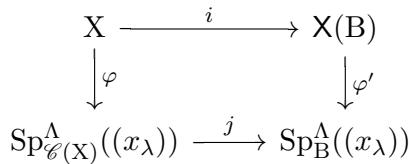
\includegraphics[keepaspectratio]{images/part001_f1662ccb.jpg}}

其中 \(\varphi\) 与 \(\varphi'\) 是由族 \((x_{\lambda})_{\lambda \in \Lambda}\) 所定义的映射（参见 I，第 41 页，第 6 节），而 \(i\) 与 \(j\) 是典范单射。则：

\begin{enumerate}
\def\labelenumi{\alph{enumi})}
\item
  映射 \(\varphi\) 与 \(\varphi'\) 是同胚；
\item
  联合谱 \(\mathrm{Sp}_{\mathrm{B}}^{\Lambda}((x_{\lambda}))\) 是 \(\mathrm{Sp}_{\mathcal{C}(\mathrm{X})}^{\Lambda}((x_{\lambda}))\) 的多项式凸包；
\item
  映射 \(\varphi\) 把 \(\mathcal{C}(\mathrm{X})\) 映为 \(\mathcal{C}(\mathrm{Sp}_{\mathcal{C}(\mathrm{X})}^{\Lambda}((x_{\lambda})))\) ，把 B 映为 \(\mathrm{P}(\mathrm{Sp}_{\mathcal{C}(\mathrm{X})}^{\Lambda}((x_{\lambda})))\) ；
\item
  映射 \(\varphi^{\prime}\) 把 \(\mathcal{G}_{\mathrm{B}}(\mathrm{B})\) 映为 \(\mathrm{P}(\mathrm{Sp}_{\mathrm{B}}^{\Lambda}((x_{\lambda})))\) ；
\item
  映射 \(\varphi\) 与 \(\varphi'\) 把 \(\mathcal{G}_{\mathrm{B}}\) 映为从 \(\mathrm{P}(\mathrm{Sp}_{\mathcal{C}(\mathrm{X})}^{\Lambda}((x_{\lambda})))\) 到 \(\mathrm{P}(\mathrm{Sp}_{\mathrm{B}}^{\Lambda}((x_{\lambda})))\) 上的典范同构。
\end{enumerate}

映射 \(\varphi\) 与 \(\varphi'\) 是连续且满射的（I，第 41 页，第 6 节）。映射 \(\varphi'\) 由 I，第 43 页，命题 12 的断言 \(a\) ）是同胚，且 \(i\) 是单射，因此 \(\varphi\) 是单射。于是 \(\varphi\) 与 \(\varphi'\) 都是同胚。

设 \(X_{1} = \mathrm{Sp}_{\mathcal{C}(X)}^{\Lambda}((x_{\lambda}))\) 。由 I，第 46 页，命题 14，\(X_{1}\) 的多项式凸包是 \(Y_{1} = \mathrm{Sp}_{\mathrm{B}}^{\Lambda}((x_{\lambda}))\) 。

对每个 \(\lambda\in\Lambda\) ，设 \(z_{\lambda}\) 是 \(\mathbf{C}^{\Lambda}\) 上相应的坐标函数。映射 \(\varphi\) 把 \(x_{\lambda}\) 映为 \(z_{\lambda}|X_{1}\) ，\(\varphi'\) 把 \(\mathcal{G}_{\mathrm{B}}(x_{\lambda})\) 映为 \(z_{\lambda}|Y_{1}\) 。因此 \(\varphi\) 把 B 映到 \(\mathrm{P}(X_{1})\) 上，\(\varphi'\) 把 \(\mathcal{G}_{\mathrm{B}}(B)\) 映到 \(\mathrm{P}(Y_{1})\) 上。最后，\(\varphi\) 与 \(\varphi'\) 把 \(\mathcal{G}_{\mathrm{B}}\) 映为从 \(\mathrm{P}(X_{1})\) 到 \(\mathrm{P}(Y_{1})\) 上的典范同构。

推论 1.　设 \(\Lambda\) 为一个集合，X 为 \(\mathbf{C}^{\Lambda}\) 的紧子集。我们把 X 等同于 \(\mathsf{X}(\mathrm{P}(\mathrm{X}))\) 的一个子集（I，第 142 页，命题 1，d)）。设 \((z_{\lambda})_{\lambda \in \Lambda}\) 为 \(\mathbf{C}^{\Lambda}\) 上坐标函数所成的族。

\begin{enumerate}
\def\labelenumi{\alph{enumi})}
\item
  映射 \(\theta\) 从 \(\mathrm{X}(\mathrm{P}(\mathrm{X}))\) 到 \(\mathrm{Sp}_{\mathrm{P}(\mathrm{X})}^{\Lambda}((z_{\lambda}))\) 上、由族 \((z_{\lambda})\) 所定义，它是从 \(\mathrm{X}(\mathrm{P}(\mathrm{X}))\) 到多项式凸包 \(Y\) （\(X\) 的多项式凸包）上的同胚。它在 \(X\) 上的限制是 \(X\) 的恒等映射；
\item
  对每个函数 \(f \in \mathrm{P}(\mathrm{X})\) ，同胚 \(\theta\) 把扩张 \(\mathcal{G}_{\mathrm{P}(\mathrm{X})}(f)\) （\(f\) 到 \(\mathrm{X}(\mathrm{P}(\mathrm{X}))\) 上的扩张）变换为扩张 \(\widetilde{f}\) （\(f\) 到 \(\mathrm{Y}\) 上的扩张）。映射 \(f \mapsto \widetilde{f}\) 是从 \(\mathrm{P}(\mathrm{X})\) 到 \(\mathrm{P}(\mathrm{Y})\) 上的典范同构。
\end{enumerate}

在命题 4 中取 B = P(X) 及 \(x_{\lambda} = z_{\lambda}\) 。则 \(\varphi\) 变成恒等映射，\(\varphi'\) 变成映射 \(\theta\) 。于是推论的断言就归结为同前处的断言。

推论 2.　设 \(\Lambda\) 为一个集合，\(X \subset \mathbf{C}^{\Lambda}\) 为紧集。若 \(X\) 连通，则它的多项式凸包连通。

若 X 连通，则 \(\mathcal{C}(\mathrm{X})\) 从而 \(\mathrm{P}(\mathrm{X})\) 的幂等元只有 0 和 1（I，第 79 页，命题的推论）。因此，空间 \(\mathrm{X}(\mathrm{P}(\mathrm{X}))\) 是连通的（同前）；而这个集合同胚于 X 的多项式凸包（推论 1，a)）。

\subsection{\texorpdfstring{\(C\) 的紧子集上的连续函数}{C 的紧子集上的连续函数}}

引理 1.　设 X 为平面的一个紧子集，O 为 \(\mathbf{C} - \mathbf{X}\) 的一个有界连通分支。则 O 的边界包含于 X。

集合 O 在 C−X 中的闭包等于 \(\overline{\mathrm{O}}\cap (\mathbf{C} - \mathbf{X})\) ，其中 \(\overline{\mathrm{O}}\) 是它在 C 中的闭包。由于 O 是 C−X 的一个连通分支，我们有 \(\overline{\mathrm{O}}\cap (\mathbf{C} - \mathbf{X}) = \mathrm{O}\) ，这确实证明了 \(\overline{\mathrm{O}} -\mathrm{O}\subset \mathrm{X}\) 。

设 X 为 C 的紧子集。设 \(O_{\infty}\) 为 \(\mathbf{C} - \mathbf{X}\) 的无界连通分支，\((\mathrm{O}_{i})_{i\in\mathrm{I}}\) 为 \(\mathbf{C} - \mathbf{X}\) 的有界连通分支的族，诸集合 \(O_{i}\) 两两不同。

设 E 为 \(\mathbf{C} - \mathbf{X}\) 的一个子集。我们用 \(\mathrm{R}_{\mathrm{E}}(\mathrm{X})\) 表示 \(\mathcal{C}(\mathrm{X})\) 中由函数 \(f|\mathrm{X}\) （其中 \(f\) 为 \(\mathbf{C}\) 上极点均属于 E 的有理函数）所成集合的闭包。代数 \(\mathrm{R}_{\mathrm{E}}(\mathrm{X})\) 是 \(\mathcal{C}(\mathrm{X})\) 的分离 X 的点的幺 Banach 子代数。设 z 是 X 上的恒等函数。\(\mathrm{R}_{\mathrm{E}}(\mathrm{X})\) 的由 z 生成的全闭子代数等于 \(\mathrm{R}_{\mathrm{E}}(\mathrm{X})\) （I，第 6 页，引理 2）。\(\mathrm{R}_{\mathrm{E}}(\mathrm{X})\) 的元素在 X 的内部全纯。

特别地，我们有 \(\mathrm{R}_{\varnothing}(\mathrm{X})=\mathrm{P}(\mathrm{X})\) 。我们记 \(\mathrm{R}(\mathrm{X})=\mathrm{R}_{\mathbf{C}-\mathbf{X}}(\mathrm{X})\) 。我们用 I(E) 表示这样的元素 \(i\in I\) 所成的集合：\(E\cap O_{i}=\varnothing\) ，并且

\[
\mathrm{X} _ {\mathrm{E}} = \mathrm{X} \cup \Big (\bigcup_ {i \in \mathrm{I} (\mathrm{E})} \mathrm{O} _ {i} \Big).
\]

集合 \(X_{E}\) 是紧的，因为它有界且闭：它在 \(\mathbf{C}\) 中的余集是开集 \(O_{\infty}\) 与诸和 E 相交的开集 \(O_{i}\) 的并。

命题 5.　沿用上述记号：

\begin{enumerate}
\def\labelenumi{\alph{enumi})}
\item
  从 \(\mathrm{R}_{\mathrm{E}}(\mathrm{X}_{\mathrm{E}})\) 到 \(\mathrm{R}_{\mathrm{E}}(\mathrm{X})\) 中的限制映射 h 是一个等距同构；
\item
  代数 \(\mathrm{R}_{\mathrm{E}}(\mathrm{X}_{\mathrm{E}})\) 是 \(\mathcal{C}(\mathrm{X}_{\mathrm{E}})\) 的全子代数；
\item
  \(\mathrm{R}_{\mathrm{E}}(\mathrm{X}_{\mathrm{E}})\) 的每个特征标都具有形式 \(f \mapsto f(w)\) ，其中 w 是 \(X_{E}\) 的元素；
\item
  映射 \(\chi \mapsto \chi (z)\) 是从 \(\mathsf{X}(\mathrm{R}_{\mathrm{E}}(\mathrm{X}))\) 到 \(\mathrm{X}_{\mathrm{E}}\) 上的同胚；
\item
  若 E′ 是 \(\mathbf{C} - \mathbf{X}\) 的子集，则我们有 \(\mathrm{R}_{\mathrm{E}}(\mathrm{X}) = \mathrm{R}_{\mathrm{E}'}(\mathrm{X})\) 当且仅当 \(\mathrm{X}_{\mathrm{E}} = \mathrm{X}_{\mathrm{E}'}\) ，这也等价于 \(\mathrm{I}(\mathrm{E}) = \mathrm{I}(\mathrm{E}')\) 。
\end{enumerate}

限制映射 \(h\) 从 \(\mathrm{R}_{\mathrm{E}}(\mathrm{X}_{\mathrm{E}})\) 到 \(\mathrm{R}_{\mathrm{E}}(\mathrm{X})\) 中，它是一个 Banach 代数态射，满足 \(\| h(f)\| \leqslant \| f\|\) 对每个函数 \(f\in \mathrm{R}_{\mathrm{E}}(\mathrm{X}_{\mathrm{E}})\) 成立。设 \(f\in \mathrm{R}_{\mathrm{E}}(\mathrm{X}_{\mathrm{E}})\) ，\(i\in \mathrm{I}(\mathrm{E})\) 。由于 \(f\) 在有界开集 \(\mathrm{O}_i\) 的一个邻域中全纯，最大模原理（VAR，I，第 29 页）蕴涵：存在元素 \(z_0\) ，它在 \(\mathrm{O}_i\) 的边界中，使得 \(|f(z_0)| = \sup_{z\in \mathrm{O}_i}|f(z)|\) 。由于 \(\mathrm{O}_i\) 的边界包含于 X（引理 1），由此得 \(\sup_{z\in \mathrm{O}_i}|f(z)|\leqslant \| h(f)\|\) 。由于这个不等式对每个 \(i\in \mathrm{I}(\mathrm{E})\) 成立，便得 \(\| f\| \leqslant \| h(f)\|\) 。因此态射 \(h\) 是等距的，特别地是单射。现在证明它是满射的。设 \(g\in \mathrm{R}_{\mathrm{E}}(\mathrm{X})\) 。存在极点都属于 E 的有理函数的序列 \((f_n)\) ，它在 X 上一致收敛于 \(g\) 。诸 \(f_n|\mathrm{X}_{\mathrm{E}}\) 是 \(\mathrm{R}_{\mathrm{E}}(\mathrm{X}_{\mathrm{E}})\) 的元素。由于 \(h\) 是等距的，序列 \((f_n|\mathrm{X}_{\mathrm{E}})\) 在 \(\mathcal{C}(\mathrm{X}_{\mathrm{E}})\) 中收敛。若 \(f\) 是它的极限，则我们有 \(f\in \mathrm{R}_{\mathrm{E}}(\mathrm{X}_{\mathrm{E}})\) 且 \(g = f|\mathrm{X} = h(f)\) 。由此得 \(a\) ）。

我们证明断言 d)。把 I，第 144 页，命题 3 应用于代数 \(B = \mathrm{R}_{\mathrm{E}}(\mathrm{X})\) 。同前处的断言 b) 蕴涵：把 \(\chi(z)\) 对应于 \(\chi\) 的映射是从 \(\mathsf{X}(\mathrm{R}_{\mathrm{E}}(\mathrm{X}))\) 到 \(\mathrm{Sp}_{\mathrm{R}_{\mathrm{E}}(\mathrm{X})}(z)\) 上的同胚。设 \(z_{\mathrm{E}}\) 为 \(\mathrm{X}_{\mathrm{E}}\) 的恒等映射。由同前处 a)，我们有 \(\mathrm{Sp}_{\mathrm{R}_{\mathrm{E}}(\mathrm{X})}(z) = \mathrm{Sp}_{\mathrm{R}_{\mathrm{E}}(\mathrm{X}_{\mathrm{E}})}(z_{\mathrm{E}})\) 。因此只需证明 \(\mathrm{Sp}_{\mathrm{R}_{\mathrm{E}}(\mathrm{X}_{\mathrm{E}})}(z_{\mathrm{E}}) = \mathrm{X}_{\mathrm{E}}\) 。I，第 28 页，命题 6 的推论表明，\(\mathrm{Sp}_{\mathrm{R}_{\mathrm{E}}(\mathrm{X}_{\mathrm{E}})}(z_{\mathrm{E}})\) 是 \(\mathrm{Sp}_{\mathcal{C}(\mathrm{X}_{\mathrm{E}})}(z_{\mathrm{E}}) = \mathrm{X}_{\mathrm{E}}\) 与 \(\mathrm{X}_{\mathrm{E}}\) 的余集的某些有界连通分支的并。设 \(\mathrm{O}_{i}\) 是 \(\mathrm{X}_{\mathrm{E}}\) 的余集的一个有界连通分支。则交 \(\mathrm{E} \cap \mathrm{O}_{i}\) 非空。设 \(\lambda \in \mathrm{E} \cap \mathrm{O}_{i}\) ；由于 \((\lambda - z_{\mathrm{E}})^{-1} \in \mathrm{R}_{\mathrm{E}}(\mathrm{X}_{\mathrm{E}})\) ，我们有 \(\lambda \notin \mathrm{Sp}_{\mathrm{R}_{\mathrm{E}}(\mathrm{X}_{\mathrm{E}})}(z_{\mathrm{E}})\) 。于是 \(\mathrm{O}_{i}\) 不包含于 \(\mathrm{Sp}_{\mathrm{R}_{\mathrm{E}}(\mathrm{X}_{\mathrm{E}})}(z_{\mathrm{E}})\) 。这就表明 \(\mathrm{Sp}_{\mathrm{R}_{\mathrm{E}}(\mathrm{X}_{\mathrm{E}})}(z_{\mathrm{E}}) = \mathrm{X}_{\mathrm{E}}\) 。

这个等式也蕴涵 \(\mathrm{Sp}_{\mathrm{R}_{\mathrm{E}}(\mathrm{X}_{\mathrm{E}})}(z_{\mathrm{E}})=\mathrm{Sp}_{\mathcal{C}(\mathrm{X}_{\mathrm{E}})}(z_{\mathrm{E}})\) 。这就建立了 I，第 41 页，命题 11 的条件 (iii)，该命题应用于 \(\mathrm{R}_{\mathrm{E}}(\mathrm{X}_{\mathrm{E}})\) 到 \(\mathcal{C}(\mathrm{X}_{\mathrm{E}})\) 中的典范单射以及元素 \(z_{\mathrm{E}}\) 。断言 b) 与 c) 就是同前处的等价条件 (i) 与 (ii)。

断言 \(d\) ）表明 \(\mathrm{X}_{\mathrm{E}} = \mathrm{X}_{\mathrm{E}'}\) ，只要 \(\mathrm{R}_{\mathrm{E}}(\mathrm{X}) = \mathrm{R}_{\mathrm{E}'}(\mathrm{X})\) 成立。反之，假设 \(\mathrm{X}_{\mathrm{E}} = \mathrm{X}_{\mathrm{E}'}\) 。把 \(\mathrm{E}'\) 换成 \(\mathrm{E} \cup \mathrm{E}'\) ，我们就可以假设 \(\mathrm{E} \subset \mathrm{E}'\) 。根据 \(b\) ），代数 \(\mathrm{R}_{\mathrm{E}}(\mathrm{X}_{\mathrm{E}})\) 是 \(\mathcal{C}(\mathrm{X}_{\mathrm{E}})\) 的全闭子代数，因而也是 \(\mathrm{R}_{\mathrm{E}'}(\mathrm{X}_{\mathrm{E}})\) 的全闭子代数。它包含 \(z_{\mathrm{E}}\) ，从而 \(\mathrm{R}_{\mathrm{E}}(\mathrm{X}_{\mathrm{E}}) = \mathrm{R}_{\mathrm{E}'}(\mathrm{X}_{\mathrm{E}})\) 。应用 \(a\) ），便推出 \(\mathrm{R}_{\mathrm{E}}(\mathrm{X}) = \mathrm{R}_{\mathrm{E}'}(\mathrm{X})\) 。最后，\(\mathrm{X}_{\mathrm{E}} = \mathrm{X}_{\mathrm{E}'}\) 与 \(\mathrm{I}(\mathrm{E}) = \mathrm{I}(\mathrm{E}')\) 的等价性是定义的直接推论。

推论 1.　下列条件等价：

\begin{enumerate}
\def\labelenumi{(\roman{enumi})}
\item
  集合 E 与 \(\mathbf{C} - \mathbf{X}\) 的每个有界连通分支相交；
\item
  映射 \(\chi \mapsto \chi (z)\) 是从 \(\mathsf{X}(\mathrm{R}_{\mathrm{E}}(\mathrm{X}))\) 到 \(\mathrm{X}\) 上的同胚；
\item
  我们有 \(\mathrm{R_E(X)} = \mathrm{R(X)}\) 。
\end{enumerate}

设 \(E' = \mathbf{C} - \mathbf{X}\) 。条件 (i)、(ii)、(iii) 分别等价于 \(\mathrm{I}(\mathrm{E}) = \mathrm{I}(\mathrm{E}')\) 、等价于 \(\mathrm{X}_{\mathrm{E}} = \mathrm{X}_{\mathrm{E}'}\) （由命题 5，d)）、等价于 \(\mathrm{R}_{\mathrm{E}}(\mathrm{X}) = \mathrm{R}_{\mathrm{E}'}(\mathrm{X})\) 。因此，由命题 5，e)，它们彼此等价。

下面的推论使 Runge 定理（I，第 69 页，定理 3）更精确。

推论 2（Runge 定理）.　对每个 \(i \in I\) ，设 \(\lambda_{i}\) 为 \(O_{i}\) 中的一点。设 f 为在 X 的一个开邻域中全纯的复函数。则 \(f|X\) 是极点取自诸 \(\lambda_{i}\) 的有理函数的限制在 X 上的一致极限。

取 \(E = \{\lambda_{i}\}_{i \in I}\) ，假设便是推论 1 的条件 (i)。因此我们有 \(\mathrm{R}_{\mathrm{E}}(\mathrm{X}) = \mathrm{R}(\mathrm{X})\) ，而 I，第 69 页，定理 3 表明 \(\mathrm{R}(\mathrm{X}) = \mathcal{O}(\mathrm{X})\) 。

\exercisesection{谱与特征标}


\begin{enumerate}
\def\labelenumi{\arabic{enumi})}
\item
  设 \((e_{1}, e_{2})\) 为 \(R^{2}\) 的典范基，u 为 A = \(\mathcal{L}(\mathbf{R}^{2})\) 中由 \(u(e_{1}) = e_{2}\) ，\(u(e_{2}) = -e_{1}\) 所定义的元素。证明 \(\mathrm{Sp}_{\mathrm{A}}(u) = \varnothing\) 与 \(\mathrm{Sp}_{\mathrm{A}}(u^{2}) = \{-1\}\) 。
\item
  设 \(\mu\) 为 \([0,1]\) 上的 Lebesgue 测度，H 为 Hilbert 空间 \(\mathrm{L}_{\mathbf{C}}^{2}([0,1],\mu)\) ，\(\mathrm{A} = \mathcal{L}(\mathrm{H})\) ，\(x \in \mathrm{A}\) 为把函数 \(f(t)\) 变换为函数 \(tf(t)\) 的算子。证明 \(\mathrm{Sp}_{\mathrm{A}}(x) = [0,1]\) ，但 \(x\) 没有特征值。
\item
  \begin{enumerate}
  \def\labelenumii{\alph{enumii})}
  \tightlist
  \item
    设 H 为具有可数正交基 \((e_{0}, e_{1}, e_{2}, \ldots)\) 的 Hilbert 空间，A = L(H)。设 \(u \in \mathcal{L}(H)\) 满足：对每个 i 有 \(u(e_{i}) = e_{i+1}\) 。设 \(u' \in \mathcal{L}(H)\) 满足：\(u'(e_{i}) = e_{i-1}\) 对 \(i \geqslant 1\) 成立，且 \(u'(e_{0}) = 0\) 。我们有 \(u'u = 1\) ，但 \(uu'(e_{0}) = 0\) ，于是 \(\mathrm{Sp}_{\mathrm{A}}(u'u) \neq \mathrm{Sp}_{\mathrm{A}}(uu')\) 。
  \end{enumerate}
\end{enumerate}

\begin{enumerate}
\def\labelenumi{\alph{enumi})}
\setcounter{enumi}{1}
\tightlist
\item
  设 A 为交换域上的幺 Noether 代数。若 \(x, y \in A\) ，则有 \(\mathrm{Sp}_{\mathrm{A}}(xy) = \mathrm{Sp}_{\mathrm{A}}(yx)\) （利用 A，VIII，第 37 页，习题 6）。
\end{enumerate}

\begin{enumerate}
\def\labelenumi{\arabic{enumi})}
\setcounter{enumi}{3}
\tightlist
\item
  设 A 为 C 上的交换代数，I 为 A 的理想，h 为 I 到 A 中的典范单射，S 为在 I 上为零的 \(\chi \in \mathsf{X}'(\mathsf{A})\) 所成的集合。
\end{enumerate}

\begin{enumerate}
\def\labelenumi{\alph{enumi})}
\item
  \(X'(h)\) 是满射的。
\item
  \(\mathsf{X}^{\prime}(h)|(\mathsf{X}^{\prime}(\mathsf{A})-\mathsf{S})\) 是从 \(\mathsf{X}^{\prime}(\mathsf{A})-\mathsf{S}\) 到 \(\mathsf{X}(\mathsf{I})\) 上的同胚。（设 \(\chi_{0}\in\mathsf{X}^{\prime}(\mathsf{A})-\mathsf{S}\) 。设 \(x_{1},\ldots,x_{n}\in\mathsf{A}\) ，\(\varepsilon>0\) ，并设 V 为 \(\chi_{0}\) 在 \(\mathsf{X}^{\prime}(\mathsf{A})\) 中由 \(|(\chi-\chi_{0})(x_{i})|\leqslant\varepsilon,(i=1,\ldots,n)\) 所定义的邻域。设 \(u_{0}\in I\) 满足 \(\chi_0(u_0) = 1\) 。我们有 \(u_i = u_0x_i \in I\) 。于是，若 \(|(\chi - \chi_0)(u_i)| \leqslant \delta\) （ \(i = 0, 1, \ldots, n\) ），其中 \(\delta\) 足够小，则我们有 \(\chi \in V\) 。）
\end{enumerate}

\begin{enumerate}
\def\labelenumi{\arabic{enumi})}
\setcounter{enumi}{4}
\item
  在习题 4 中，取 \(A = \mathbf{C}[X,Y]\) 与 \(I = AX\) 。空间 X(A) 等同于 \(\mathbf{C}^2\) ，S = \{0\} 等同于 \(\{0\} \times \mathbf{C}\) 。设 U 为这样的 \((\xi, \eta) \in \mathbf{C}^2\) 所成的集合：\(|\xi| < e^{-|\eta|}\) 。证明 \(X'(h)(U)\) 不是 0 在 \(X'(I)\) 中的邻域。由此推出，\(X'(I)\) 不能等同于 \(X'(A)\) 关于由 \(X'(h)\) 所定义的等价关系的商空间。（关于这一主题，参见 I，第 169 页，习题 17。）
\item
  设 A 为域上的交换代数，I 为 A 的极大理想。证明我们有 \(A^{2} \subset I\) 且 \(\dim(A/I) = 1\) ，或者 A/I 是一个域。（对 A/I 应用 A，I，第 153 页，习题 3。）特别地，若 \(A^{2} = A\) ，则 A 的每个极大理想都是正则的。
\item
  设 A 为交换域 K 上的交换代数，\(x \in A\) ，\(\alpha \in K\) 。这样的 \(\chi \in \mathsf{X}(\mathsf{A})\) 所成的集合：\((\mathcal{G}x)(\chi) = \alpha\) ，它在 Jacobson 拓扑下是闭的。（先归结为 A 有单位元的情形，再归结为 \(\alpha = 0\) 的情形。）
\end{enumerate}

¶ 8) 设 A 为一个代数，I 为 A 的双边理想，\(\mathrm{J}^{\mathrm{I}}(\mathrm{A})\) 为 A 的不包含 I 的本原理想所成的集合，\(\widehat{A}^{I}\) 为不可约表示 \(\pi \in \widehat{A}\) （满足 \(\pi(I) \neq 0\) ）所成的集合。

\begin{enumerate}
\def\labelenumi{\alph{enumi})}
\item
  若 \(\pi \in \widehat{\mathrm{A}}^{\mathrm{I}}\) ，则 \(\pi | \mathrm{I} \in \widehat{\mathrm{I}}\) （I，第 12 页，引理 5，\(a\) ））。若表示 \(\pi\) 与 \(\pi' \in \widehat{\mathrm{A}}\) 使得 \(\pi | \mathrm{I}\) 与 \(\pi'|\mathrm{I}\) 等价，则 \(\pi\) 与 \(\pi'\) 等价。（可以假设 \(\pi(x) = \pi'(x)\) 对所有 \(x \in \mathrm{I}\) 成立。于是，对每个 \(y \in \mathrm{A}\) ，\(\pi(y)\) 与 \(\pi'(y)\) 在 \(\sum_{x \in \mathrm{I}} \operatorname{Im} \pi(x)\) 上一致，而这个子空间等于 \(\pi\) 的空间。）
\item
  若 \(\pi \in \widehat{\mathrm{I}}\) ，则 \(\pi\) 可扩张为 \(\widehat{\mathrm{A}}^{\mathrm{I}}\) 的一个元素。（设 R 为 I 的极大正则左理想。设 \(g\) 为 I 模 R 的右单位元。假设 A 有单位元，证明关系式 \(\mathrm{AR} + \mathrm{A}(1 - g) = \mathrm{A}\) 将导出 \(g^2 \in \mathrm{R}\) 。因此 \(\mathrm{AR} + \mathrm{A}(1 - g)\) 包含于 A 的一个极大左理想 M。证明 \(\mathrm{M} \cap \mathrm{I} = \mathrm{R}\) 与 \(\mathrm{M} + \mathrm{I} = \mathrm{A}\) 。）
\item
  由 a) 与 b) 推出：映射 \(I'\mapsto I'\cap I\) 是从 \(\mathrm{J}^{\mathrm{I}}(\mathrm{A})\) 到 \(\mathrm{J}(\mathrm{I})\) 上的同胚，且映射 \(\pi\mapsto\pi|I\) 是从 \(\widehat{A}^{I}\) 到 \(\widehat{I}\) 上的同胚。
\end{enumerate}
